% ============================================================
% CDS533 Assignment 3 - Group report (MASTER FILE)
% OWNER: B only. Other members: do NOT edit this file.
% Revised on 23 November 2026 to match the updated Q4 R outputs.
%
%   division.tex       - B    cover + Division of Work
%   q1.tex             - A    Question 1
%   q2.tex             - A    Question 2
%   q3_abcd.tex        - B    Question 3, Studies A-D
%   q3_efg.tex         - C    Question 3, Studies E-G
%   q4_eda.tex         - D    Question 4: 1(a) 1(b) EDA + research question
%   q4_variables.tex   - C    Question 4: 2 variable types and roles
%   q4_predictors.tex  - D    Question 4: 3(a) 3(b) predictor reasoning
%   q4_models.tex      - E    Question 4: 3(c) 3(d) 3(e) models
%   references.tex     - B    sources + AI-assistance disclosure
%
% Group conventions (agreed):
%   1. NO \documentclass / \usepackage inside section files.
%   2. Tables: booktabs three-line style. Numbers to 3 decimals;
%      p < 0.001 written as "$p < 0.001$".
%   3. Figures keep the repo figures/ file names; captions keep the
%      member's own figure numbering (Figure Q1-1, Q4-D1, ...).
% ============================================================
\documentclass[11pt,a4paper]{article}

% ---------- packages (central; do not duplicate elsewhere) ----------
\usepackage[margin=1in]{geometry}
\usepackage{amsmath,amssymb}
\usepackage{graphicx}          % \includegraphics
\usepackage[section]{placeins}
\usepackage{booktabs}          % three-line tables
\usepackage[labelfont=bf]{caption}
\usepackage[colorlinks=true,linkcolor=blue,citecolor=blue,urlcolor=blue]{hyperref}

% ---------- shared notation macros ----------
\newcommand{\chisq}{\chi^2}     % e.g. $\chisq(2) = 8.202$
\newcommand{\pval}{\mathit{p}} % e.g. $\pval = 0.017$
\newcommand{\Hnull}{H_0}
\newcommand{\Halt}{H_1}

\graphicspath{{figures/}}

\setlength{\emergencystretch}{2em}
\begin{document}

\begin{center}
{\LARGE\bfseries Statistics for Data Science --- Assignment 3}\\[6pt]
{\large Group Assignment}\\[4pt]
{\normalsize November 2026}
\end{center}
\section*{Division of Work}
\begin{itemize}\setlength\itemsep{3pt}
\item \textbf{LING Tong} --- 3162677 --- Question 1 and Question 2; submission-requirements check; cross-review of Studies A--D.
\item \textbf{CHEN Yanwu} --- 3162744 --- Studies A--D (Q3); report integration and progress tracking; review of numerical results and report consistency.
\item \textbf{CHEN Yinan} --- 3162550 --- Studies E--G (Q3); QQ data preparation and variable classification; R-script integration.
\item \textbf{ZHANG Yijie} --- 3162641 --- Question 4: exploratory data analysis, predictor reasoning, correlations and multicollinearity.
\item \textbf{HU Zhongyuan} --- 3162304 --- Question 4: model comparison, diagnostics, prediction and conclusion.
\end{itemize}

% q1.tex - Question 1 (OWNER: A) - prose integrated verbatim from docs/A_Q1.md
\section{Question 1: Choosing an Advertisement}

The 34 response scores were entered value by value from the original assignment text. All values are numeric and no group contains missing values (verified using \texttt{is.na()} in R); no observations were excluded, imputed, or modified. The score of 55 in the White group is a plausibly observed low response rather than an invalid entry, and it was retained.

\subsection*{(a) Response scale, design and choice of test}

The response is measured on an ordinal scale: the question explicitly states that the response is an ordered reaction score---the values are ranked in order, but the differences between scores do not carry a strict numerical meaning, since the score is an evaluation of the advertisement. There are three groups (Red, White and Blue). The observations are independent: consumers selected at random are each shown only one advertisement, so the design is independent rather than paired. With an ordinal response, three independent groups, and no normality assumption required, the appropriate method is the Kruskal--Wallis test. The hypotheses are

\[
\Hnull\colon \text{the score distributions are identical across the three advertisements,}
\]
\[
\Halt\colon \text{at least one advertisement has a different distribution } (\alpha = 0.05).
\]

\subsection*{(b) Descriptives, plot and test}

Figure Q1-1 shows a box plot of the three advertisement response scores: White has the highest median, followed by Red and Blue; the group means follow the same order. The Kruskal--Wallis test yields $\chisq(2) = 8.202$, $\pval = 0.017$. Since $\pval < 0.05$, we reject $\Hnull$ and conclude that consumer responses to the three advertisements are not all identical.

\begin{figure}[htbp]
  \centering
  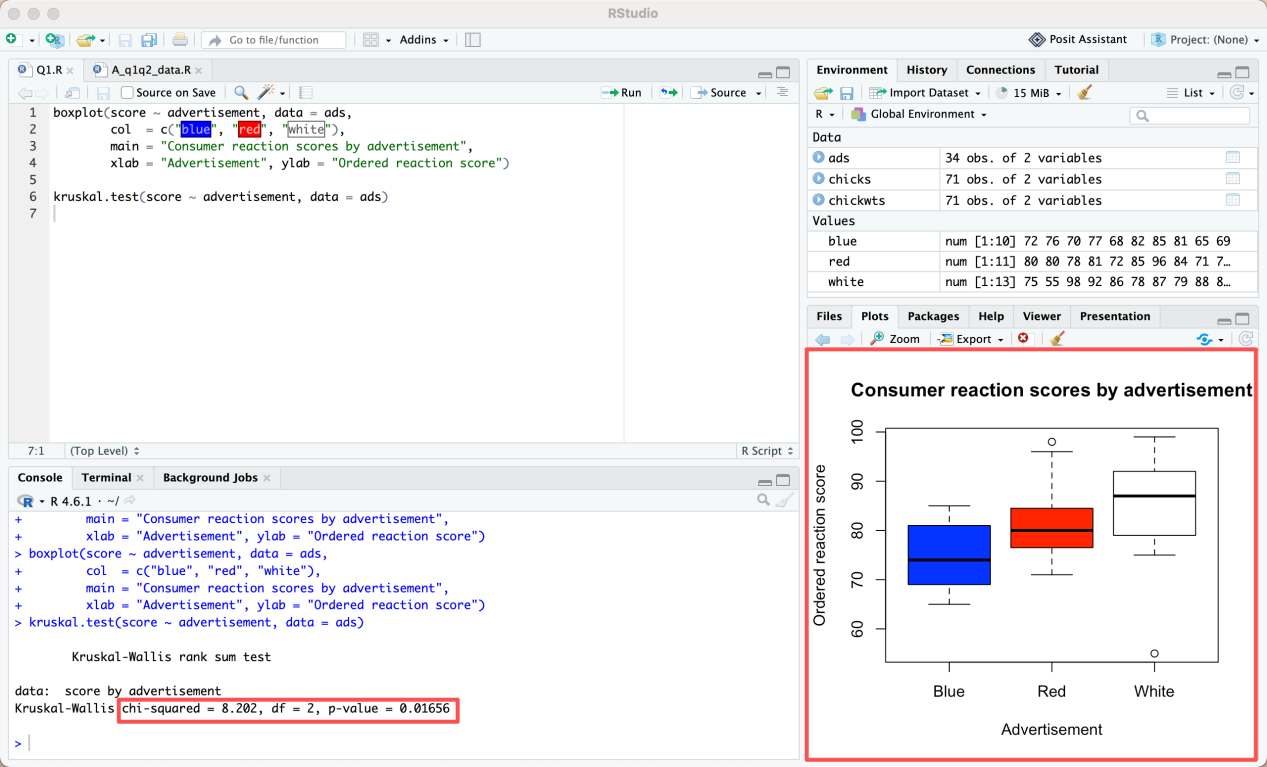
\includegraphics[width=0.85\textwidth]{Q1-1_screenshot.png}
  \caption*{Figure Q1-1: Consumer reaction scores by advertisement: boxplot and Kruskal--Wallis test output in RStudio ($n = 34$).}
\end{figure}

\subsection*{(c) Recommendation and what the overall test cannot establish}

We recommend White: it has the highest median in the descriptive statistics, and the overall test is significant, indicating that the difference is unlikely to be due to chance. Two limitations should be noted. First, the Kruskal--Wallis test is an omnibus test: it can only conclude that at least one group differs, but cannot specify which pairs differ---whether White is significantly better than Red was not tested in this question (post-hoc tests would be required to identify specific pairs). Second, the White group exhibits the greatest internal variability, so its stability is inferior to that of Red; if the team prioritises a stable, upper-middle response, Red is the defensible conservative choice. Blue ranks lowest on both kinds of evidence.

% q2.tex - Question 2 (OWNER: A) - revised from docs/A_Q2.md
\section{Question 2: Which Feed Helps Chicks Grow?}

The \texttt{chickwts} dataset is complete with 71 observations and no missing values on either variable. All 71 chicks were retained in the analysis; the residual degrees of freedom ($65 = 71 - 6$) confirm that the full sample entered the model.

\FloatBarrier
\subsection*{(a) Hypotheses and assumptions}

Let $\mu_i$ denote the population mean of the body weight of chicks after six weeks of being fed the feed $i$ ($i =$ casein, horsebean, linseed, meatmeal, soybean, sunflower).

\[
\Hnull\colon \mu_1 = \mu_2 = \mu_3 = \mu_4 = \mu_5 = \mu_6
\]
\[
\Halt\colon \text{At least one feed has a different population mean. } (\alpha = 0.05)
\]

Three main assumptions apply.

\textbf{Independence:} The observations should not influence one another, within or between groups. This assumption is supported by the study design rather than by a statistical test: newly hatched chicks were randomly allocated to the six feed groups, and each chick is an independent experimental unit.

\textbf{Normality:} The weights within each feed group should be approximately normally distributed. This is assessed from the data: a Shapiro--Wilk test on the ANOVA residuals gives $W = 0.986$, $\pval = 0.627$, and the residual Q--Q plot (Figure Q2-2) shows the points lying close to the reference line with no systematic departure. Approximate normality is therefore reasonable.

\textbf{Homogeneity of variance:} The six population variances should be equal. This is checked with Levene's test centred on group medians (the default in the \texttt{car} package), $F(5, 65) = 0.749$, $\pval = 0.590$; the mean-centred version gives $F = 0.987$, $\pval = 0.432$, with the same conclusion. Neither version rejects equal variances.

The design and diagnostics provide reasonable support for a one-way ANOVA; non-significant diagnostic tests do not prove that its assumptions hold exactly.

\FloatBarrier
\subsection*{(b) Plot, ANOVA table and decision}

\begin{table}[htbp]
  \centering
  \caption*{Table Q2-1: One-way ANOVA of six-week chick weight by feed supplement.}
  \begin{tabular}{lrrrrl}
    \toprule
    Source & df & SS & MS & $F$ & $\pval$ \\
    \midrule
    Feed & 5 & 231129 & 46226 & 15.365 & $< 0.001$ \\
    Residuals & 65 & 195556 & 3009 & & \\
    Total & 70 & 426685 & & & \\
    \bottomrule
  \end{tabular}
\end{table}

Figure Q2-1 (labelled boxplot of weight by feed) shows the highest weights under casein and sunflower and clearly lower weights under horsebean. The one-way ANOVA table (Table Q2-1) gives SS(feed) $= 231129$ on 5 df, SS(residuals) $= 195556$ on 65 df, MS(feed) $= 46226$, MS(residuals) $= 3009$, $F(5, 65) = 15.365$ with $\pval < 0.001$. Since $\pval < 0.05$ we reject $\Hnull$ and conclude that the six feed types do not all have the same population mean chick weight after six weeks; feed explains about 54.2\% of the variation in weight ($R^2 = \text{SS(feed)}/\text{SS(total)} = 231129/426685 = 0.542$). Which particular feeds differ would require post-hoc comparisons, which are beyond the required scope.

\begin{figure}[htbp]
  \centering
  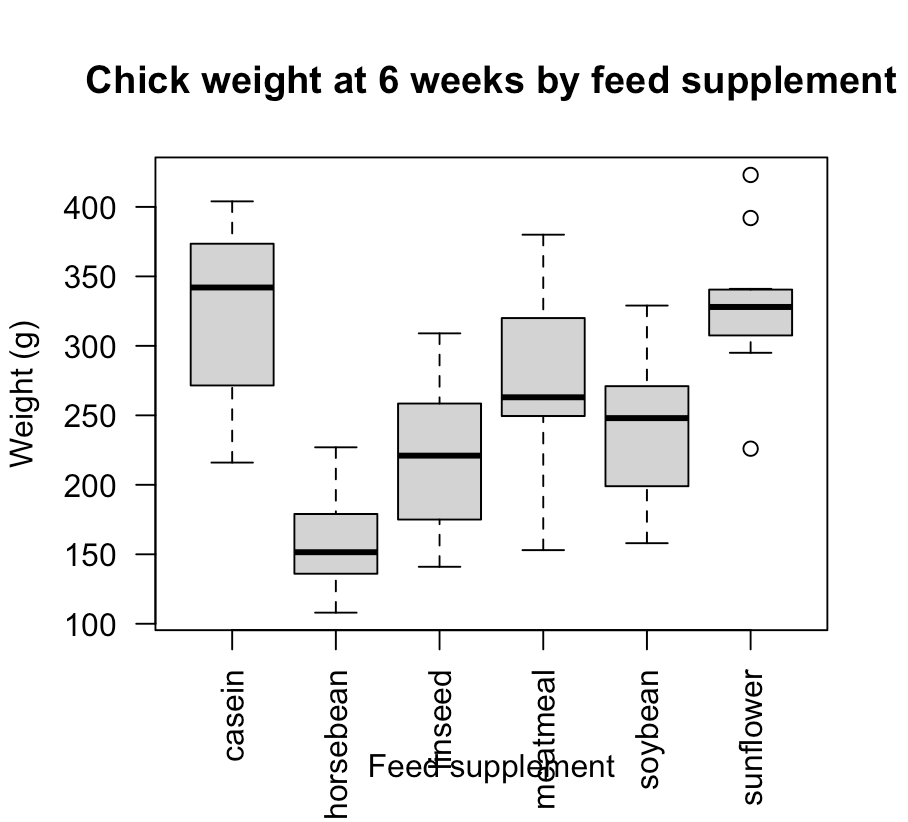
\includegraphics[width=0.75\textwidth]{Q2-1_boxplot.png}
  \caption*{Figure Q2-1: Labelled boxplot of chick weight by feed supplement.}
\end{figure}

\begin{figure}[htbp]
  \centering
  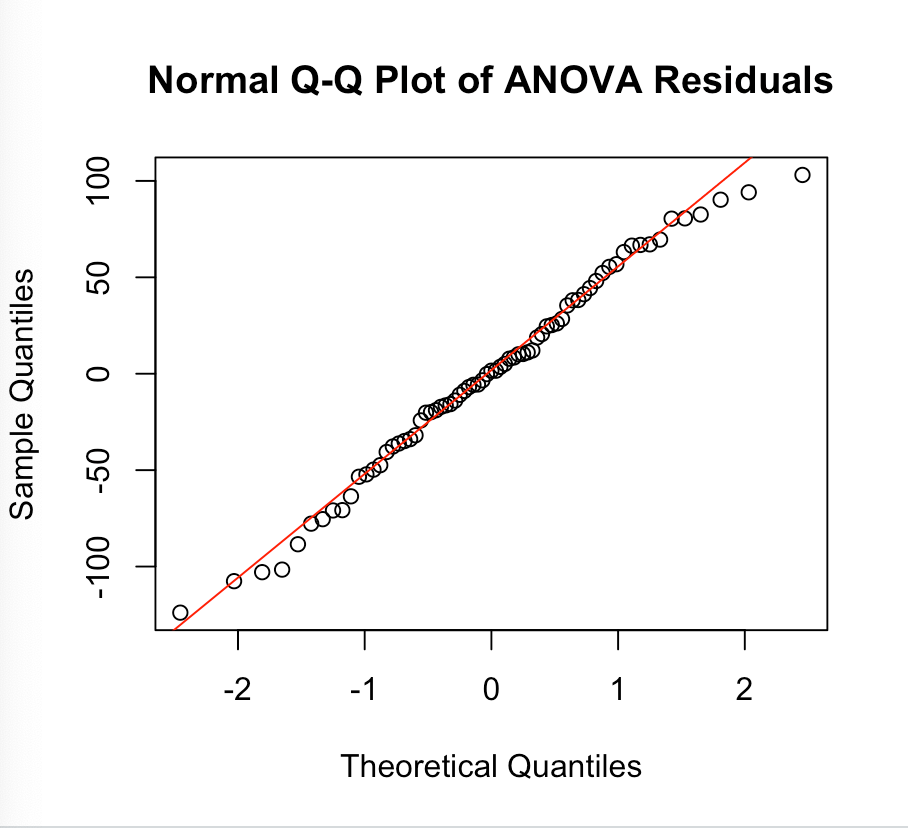
\includegraphics[width=0.6\textwidth]{Q2-2_qqplot.png}
  \caption*{Figure Q2-2: Residual Q--Q plot for the one-way ANOVA.}
\end{figure}

\FloatBarrier
\subsection*{(c) Interpretation of the claim}

This argument does not hold. A significant ANOVA F-test is an omnibus result: it only rejects the null hypothesis that ``all six population means are equal,'' establishing that ``at least one feed is different,'' but it does not establish that ``each feed is different from every other feed.'' For example, a data pattern where ``five feeds share the same mean and only one is lower'' would also yield a significant F-statistic.

The highest sample mean does not imply that it is significantly superior to all other groups: sunflower (328.9 g) exceeded casein (323.6 g) by only 5.3 g, while within-group variation is substantial. This descriptive ranking alone does not establish a statistically significant pairwise difference.

A reliable conclusion that can be drawn from this analysis is that the average weights of the six feeds are not all equal ($F(5, 65) = 15.365$, $\pval < 0.001$); descriptive evidence indicates that the weight for horsebean is lower, while those for sunflower and casein are higher. To identify which specific pairings differ, we would need to perform post-hoc multiple comparisons, such as Tukey's HSD, which controls the family-wise error rate across all 15 pairwise comparisons; however, this is not required for this problem.

% q3_abcd.tex - Question 3 Studies A-D (OWNER: B) - prose integrated verbatim from docs/B_Q3_ABCD.md
\section{Question 3, Studies A--D}

All tests are two-sided with $\alpha = 0.05$ and 95\% confidence intervals. Every test call is the version taught in the course slides (Weeks 6--8). Each study keeps the full set of records defined by the assignment's own filtering code, and the four studies answer their own questions: Study A and B target population means, Study C a sign probability, Study D whole distributions --- the four are not interchangeable conclusions.

\subsection*{Study A --- Is there a league salary gap?}

\textbf{Design.} The response is the natural log of 1987 salary, a quantitative variable; the two leagues are independent groups. Of 322 players, 59 have missing salaries and none has a non-positive salary, leaving $n = 139$ American and $n = 124$ National. $\Hnull$: the two population mean log salaries are equal; $\Halt$: they differ.

\textbf{Method.} Shapiro--Wilk rejects normality in both groups ($W = 0.974$, $\pval = 0.009$; $W = 0.962$, $\pval = 0.002$), but both samples are large (Week 6: $n \geq 30$, CLT) and the question asks about the population \emph{mean}, so a two-sample t-test is the course method here. The Week 7 F-test for equal variances gave $F(138, 123) = 1.031$, $\pval = 0.867$, so there is no evidence against equal variances and the pooled t-test is used.

\textbf{Result.} $t(261) = 0.104$, $\pval = 0.917$, 95\% CI for the difference in means $[-0.205,\ 0.228]$. Group means are nearly identical (5.933 vs 5.921). We fail to reject $\Hnull$: the data provide no evidence of a league gap in mean log salary. On the salary scale the interval corresponds to a multiplicative factor between about 0.81 and 1.26, so a practically meaningful gap in either direction is not supported either.

\begin{figure}[htbp]
  \centering
  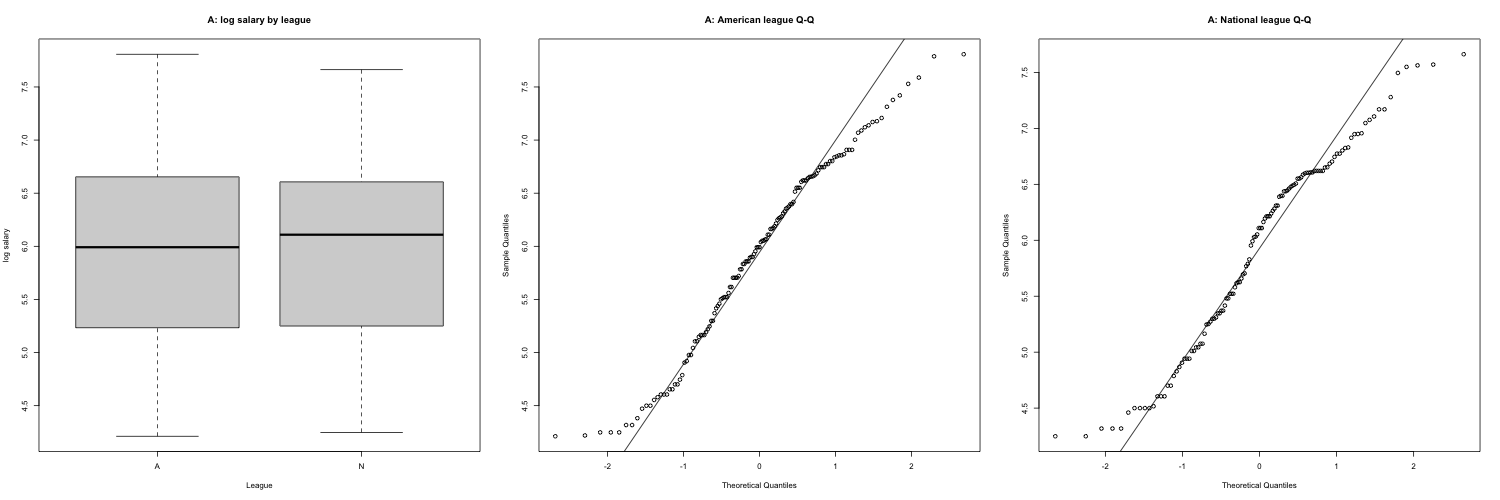
\includegraphics[width=\textwidth]{Q3_A_diagnostics.png}
  \caption*{Study A diagnostics: boxplot and Q--Q plots.}
\end{figure}

\subsection*{Study B --- Tuition versus living costs}

\textbf{Design.} Each college contributes both measurements, so the design is paired; all 777 colleges are retained (no missing or non-positive values). The response is the difference $\log(\text{Outstate}) - \log(\text{Room.Board})$. $\Hnull$: the population mean difference is zero; $\Halt$: it is not.

\textbf{Method.} Following the Week 8 pattern, the differences were checked first: Shapiro--Wilk rejects strict normality ($W = 0.987$, $\pval < 0.001$), but with 777 pairs ($n \geq 30$, CLT) and a mean-difference question, the Week 7 paired t-test is the course method.

\textbf{Result.} The mean log difference is 0.828 (SD 0.304), $t(776) = 75.774$, $\pval < 0.001$, 95\% CI $[0.806,\ 0.849]$. We reject $\Hnull$. Out-of-state tuition is clearly the larger bill: $\exp(0.828) \approx 2.29$, so tuition is on average about 2.3 times room-and-board costs, with the interval corresponding to factors from 2.24 to 2.34.

\begin{figure}[htbp]
  \centering
  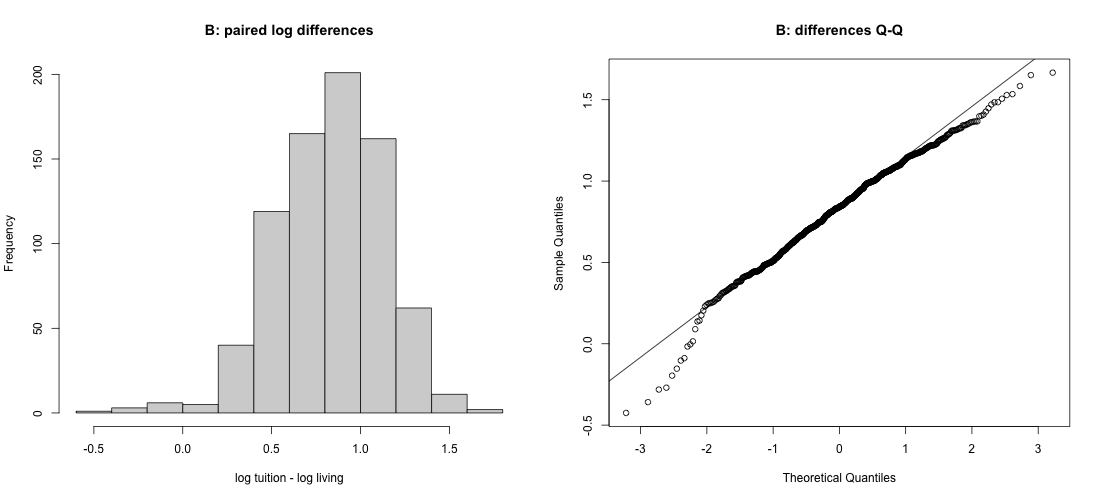
\includegraphics[width=0.9\textwidth]{Q3_B_diagnostics.png}
  \caption*{Study B diagnostics: histogram and Q--Q plot of the paired differences.}
\end{figure}

\subsection*{Study C --- Which bill is more often larger?}

\textbf{Design.} Same 777 colleges, but only the sign of Outstate $-$ Room.Board matters: 767 positive, 10 negative, 0 ties. $\Hnull$: among colleges where the two costs differ, $P(\text{tuition} > \text{room-and-board}) = 0.5$; $\Halt$: the probability differs from 0.5.

\textbf{Method.} This is a sign test, done with the Week 6 one-sample proportion test \texttt{prop.test(x, n, p = 0.5)}. It uses only the counts of positive and negative differences, so it assumes nothing about the shape of the cost distributions --- exactly what the question requires.

\textbf{Result.} $\hat{p} = 0.987$, 95\% CI $[0.976,\ 0.993]$, $\chisq(1) = 735.570$ with continuity correction, $\pval < 0.001$. We reject $\Hnull$: at almost every college, tuition is the larger bill. An exact binomial test was run as a cross-check and gives the same decision, but the course method is what is reported here.

\textbf{Compared with Study B.} Study B asks how large the gap is on average (a mean log difference); Study C asks only which side is larger (a probability). The two can disagree in principle --- a large-but-balanced gap would make B significant and C not --- but here they agree: tuition is both consistently the larger bill and much larger on average. C says nothing about magnitude, B says nothing about consistency; together they describe the gap fully.

\subsection*{Study D --- American versus Japanese fuel economy}

\textbf{Design.} mpg is quantitative; the two origin groups are independent ($n = 245$ American, $n = 79$ Japanese; all 324 retained cars have valid mpg). $\Hnull$: the two mpg distributions are identical; $\Halt$: they differ.

\textbf{Method.} Week 8 flow: Shapiro--Wilk per group rejects normality for American cars ($W = 0.934$, $\pval < 0.001$), so the two-sample t-test is not appropriate for comparing distributions; the Mann--Whitney U test (Wilcoxon rank-sum) is used instead. mpg contains tied values, so R automatically uses the normal approximation of W with continuity correction.

\textbf{Result.} $W = 2456.5$, $\pval < 0.001$. We reject $\Hnull$: the distributions differ. Japanese cars have systematically higher fuel economy --- median 31.6 mpg (IQR 8.4) versus 18.5 (IQR 9.0) for American cars. As in any observational comparison of groups, this is a difference between the cars in this 1993-era dataset, not an effect of origin itself.

\begin{figure}[htbp]
  \centering
  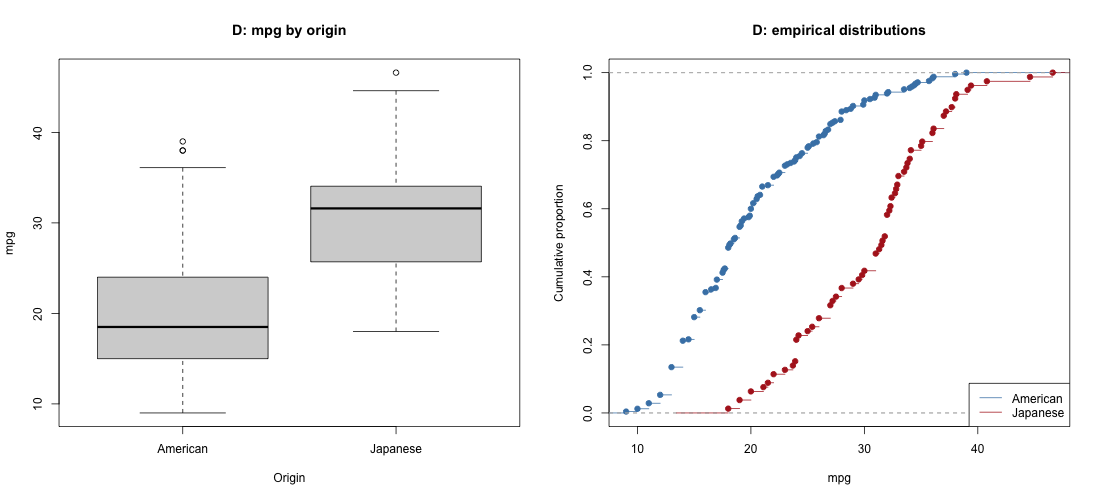
\includegraphics[width=0.9\textwidth]{Q3_D_distributions.png}
  \caption*{Study D diagnostics: boxplot and empirical CDFs.}
\end{figure}

% q3_efg.tex - Question 3 Studies E-G (OWNER: C) - revised from docs/C_Q3_EFG.md
\section{Question 3, Studies E--G}

All tests use $\alpha = 0.05$. Each study uses the complete set of records available in the named dataset for its analysis variables.

\FloatBarrier
\subsection*{Study E --- Representation of public and private colleges}

\texttt{Private} is a nominal variable with two categories. Each college is treated as an independent observation. Using all 777 colleges in \texttt{ISLR2::College}, a chi-square goodness-of-fit test compares the observed counts with a specified 50:50 split. The null hypothesis ($\Hnull$) assigns a probability of 0.5 to each category. The alternative ($\Halt$) allows the probabilities to differ from 0.5.

\begin{table}[htbp]
  \centering
  \caption*{Table Q3-E. Observed and expected college counts}
  \begin{tabular}{lrr}
    \toprule
    College type & Observed & Expected under $\Hnull$ \\
    \midrule
    Public & 212 & 388.5 \\
    Private & 565 & 388.5 \\
    \bottomrule
  \end{tabular}
\end{table}

Both expected counts exceed 5. The test gave $\chisq(1) = 160.372$, $\pval < 0.001$. We reject $\Hnull$. The data provide strong evidence against a 50:50 split. Private colleges account for 72.72\% of the records.

\FloatBarrier
\subsection*{Study F --- College status and incoming student profile}

\texttt{Private} and the High/Lower student profile are categorical variables. A college is classified as High if at least 50\% of its incoming students were in the top 10\% of their high school class. Using the same 777 colleges, we apply Pearson's chi-square test of independence without Yates' correction, treating colleges as independent observations. $\Hnull$ states that college status and student profile are independent. $\Halt$ states that they are associated.

\begin{table}[htbp]
  \centering
  \caption*{Table Q3-F. Student profile by college type}
  \begin{tabular}{lrrr}
    \toprule
    College type & Lower & High & Percent High \\
    \midrule
    Public & 198 & 14 & 6.60\% \\
    Private & 496 & 69 & 12.21\% \\
    \bottomrule
  \end{tabular}
\end{table}

The minimum expected count was 22.65. The test gave $\chisq(1) = 5.083$, $\pval = 0.024$. We reject $\Hnull$. The proportion of colleges classified as High was 12.21\% among private colleges and 6.60\% among public colleges. Study E tests whether a single variable follows a specified distribution, while Study F tests for an association between two variables. Because this is an observational comparison, the difference cannot be attributed to private status alone. Admissions selectivity, for example, may also contribute.

\FloatBarrier
\subsection*{Study G --- Variability in fuel economy by vehicle origin}

Fuel economy (\texttt{mpg}) is a quantitative ratio variable. Vehicle origin is nominal, with three groups treated as independent. Using all 392 vehicles in \texttt{ISLR2::Auto}, we apply a median-centred Levene test, which compares variability across groups without requiring normally distributed mpg. $\Hnull$ states that the three population variances are equal. $\Halt$ states that at least one differs.

\begin{table}[htbp]
  \centering
  \caption*{Table Q3-G. Fuel economy variance by origin}
  \begin{tabular}{lrr}
    \toprule
    Origin & Sample size & Sample variance (mpg$^2$) \\
    \midrule
    American & 245 & 41.479 \\
    European & 68 & 43.299 \\
    Japanese & 79 & 37.089 \\
    \bottomrule
  \end{tabular}
\end{table}

The test gave $F(2, 389) = 0.086$, $\pval = 0.918$. We fail to reject $\Hnull$. Although the European group had the largest sample variance, the test provides insufficient evidence of a difference in population variances across the three origins.

% q4_eda.tex - Question 4 parts 1(a) 1(b) (OWNER: D) - prose integrated verbatim from report/Q4_D_report_final.md
\section{Question 4: What Makes a Hit? Exploring QQ Music}

\subsection*{4.1(a) Data and exploratory analysis}

The supplied dataset contains 844 song records. We used C's trial\_v1 working data. One invalid text value in streams was recorded as missing. We selected six candidate predictors and one response variable, retaining 843 records with complete values for these variables. Records with a blank key were retained because key was not included in this analysis. All the figures, summary statistics, correlations and variance inflation factors below are based on the same 843 records.

\begin{table}[htbp]
  \centering
  \small
  \caption*{Table Q4-D1: Descriptive statistics of the analysis variables ($n = 843$).}
  \setlength{\tabcolsep}{3.5pt}
  \begin{tabular}{lrrrrrrrr}
    \toprule
    Variable & $N$ & Mean & SD & Min & Q1 & Median & Q3 & Max \\
    \midrule
    Streams (million) & 843 & 536.062 & 584.495 & 0.003 & 147.040 & 301.052 & 703.736 & 3703.895 \\
    ln(streams) & 843 & 19.541 & 1.169 & 7.924 & 18.806 & 19.523 & 20.372 & 22.033 \\
    QQ playlist inclusions & 843 & 5531.019 & 8268.126 & 31 & 895 & 2313 & 6077 & 52898 \\
    ln(QQ playlist inclusions) & 843 & 7.774 & 1.342 & 3.434 & 6.797 & 7.746 & 8.712 & 10.876 \\
    Artist count & 843 & 1.515 & 0.842 & 1 & 1 & 1 & 2 & 8 \\
    Release year & 843 & 2018.053 & 11.067 & 1942 & 2020 & 2022 & 2022 & 2023 \\
    Danceability (0--100) & 843 & 66.471 & 14.850 & 23 & 56 & 68 & 78 & 96 \\
    Energy (0--100) & 843 & 63.745 & 16.692 & 9 & 53 & 65 & 76.5 & 97 \\
    Acousticness (0--100) & 843 & 27.000 & 26.334 & 0 & 5 & 17 & 43 & 97 \\
    \bottomrule
  \end{tabular}
\end{table}

Table Q4-D1 shows that the mean total streams is 536.062 million and the median is 301.052 million. Figure Q4-D1 shows that the distribution is strongly right-skewed, with a small number of songs having very high stream counts. After applying a natural logarithm transformation, the long upper tail is compressed and most observations form a more compact cluster (see Figure Q4-D2). However, a few very low values remain in the left tail. These records were retained. The histogram alone does not indicate whether the regression assumptions are met.

\begin{figure}[htbp]
  \centering
  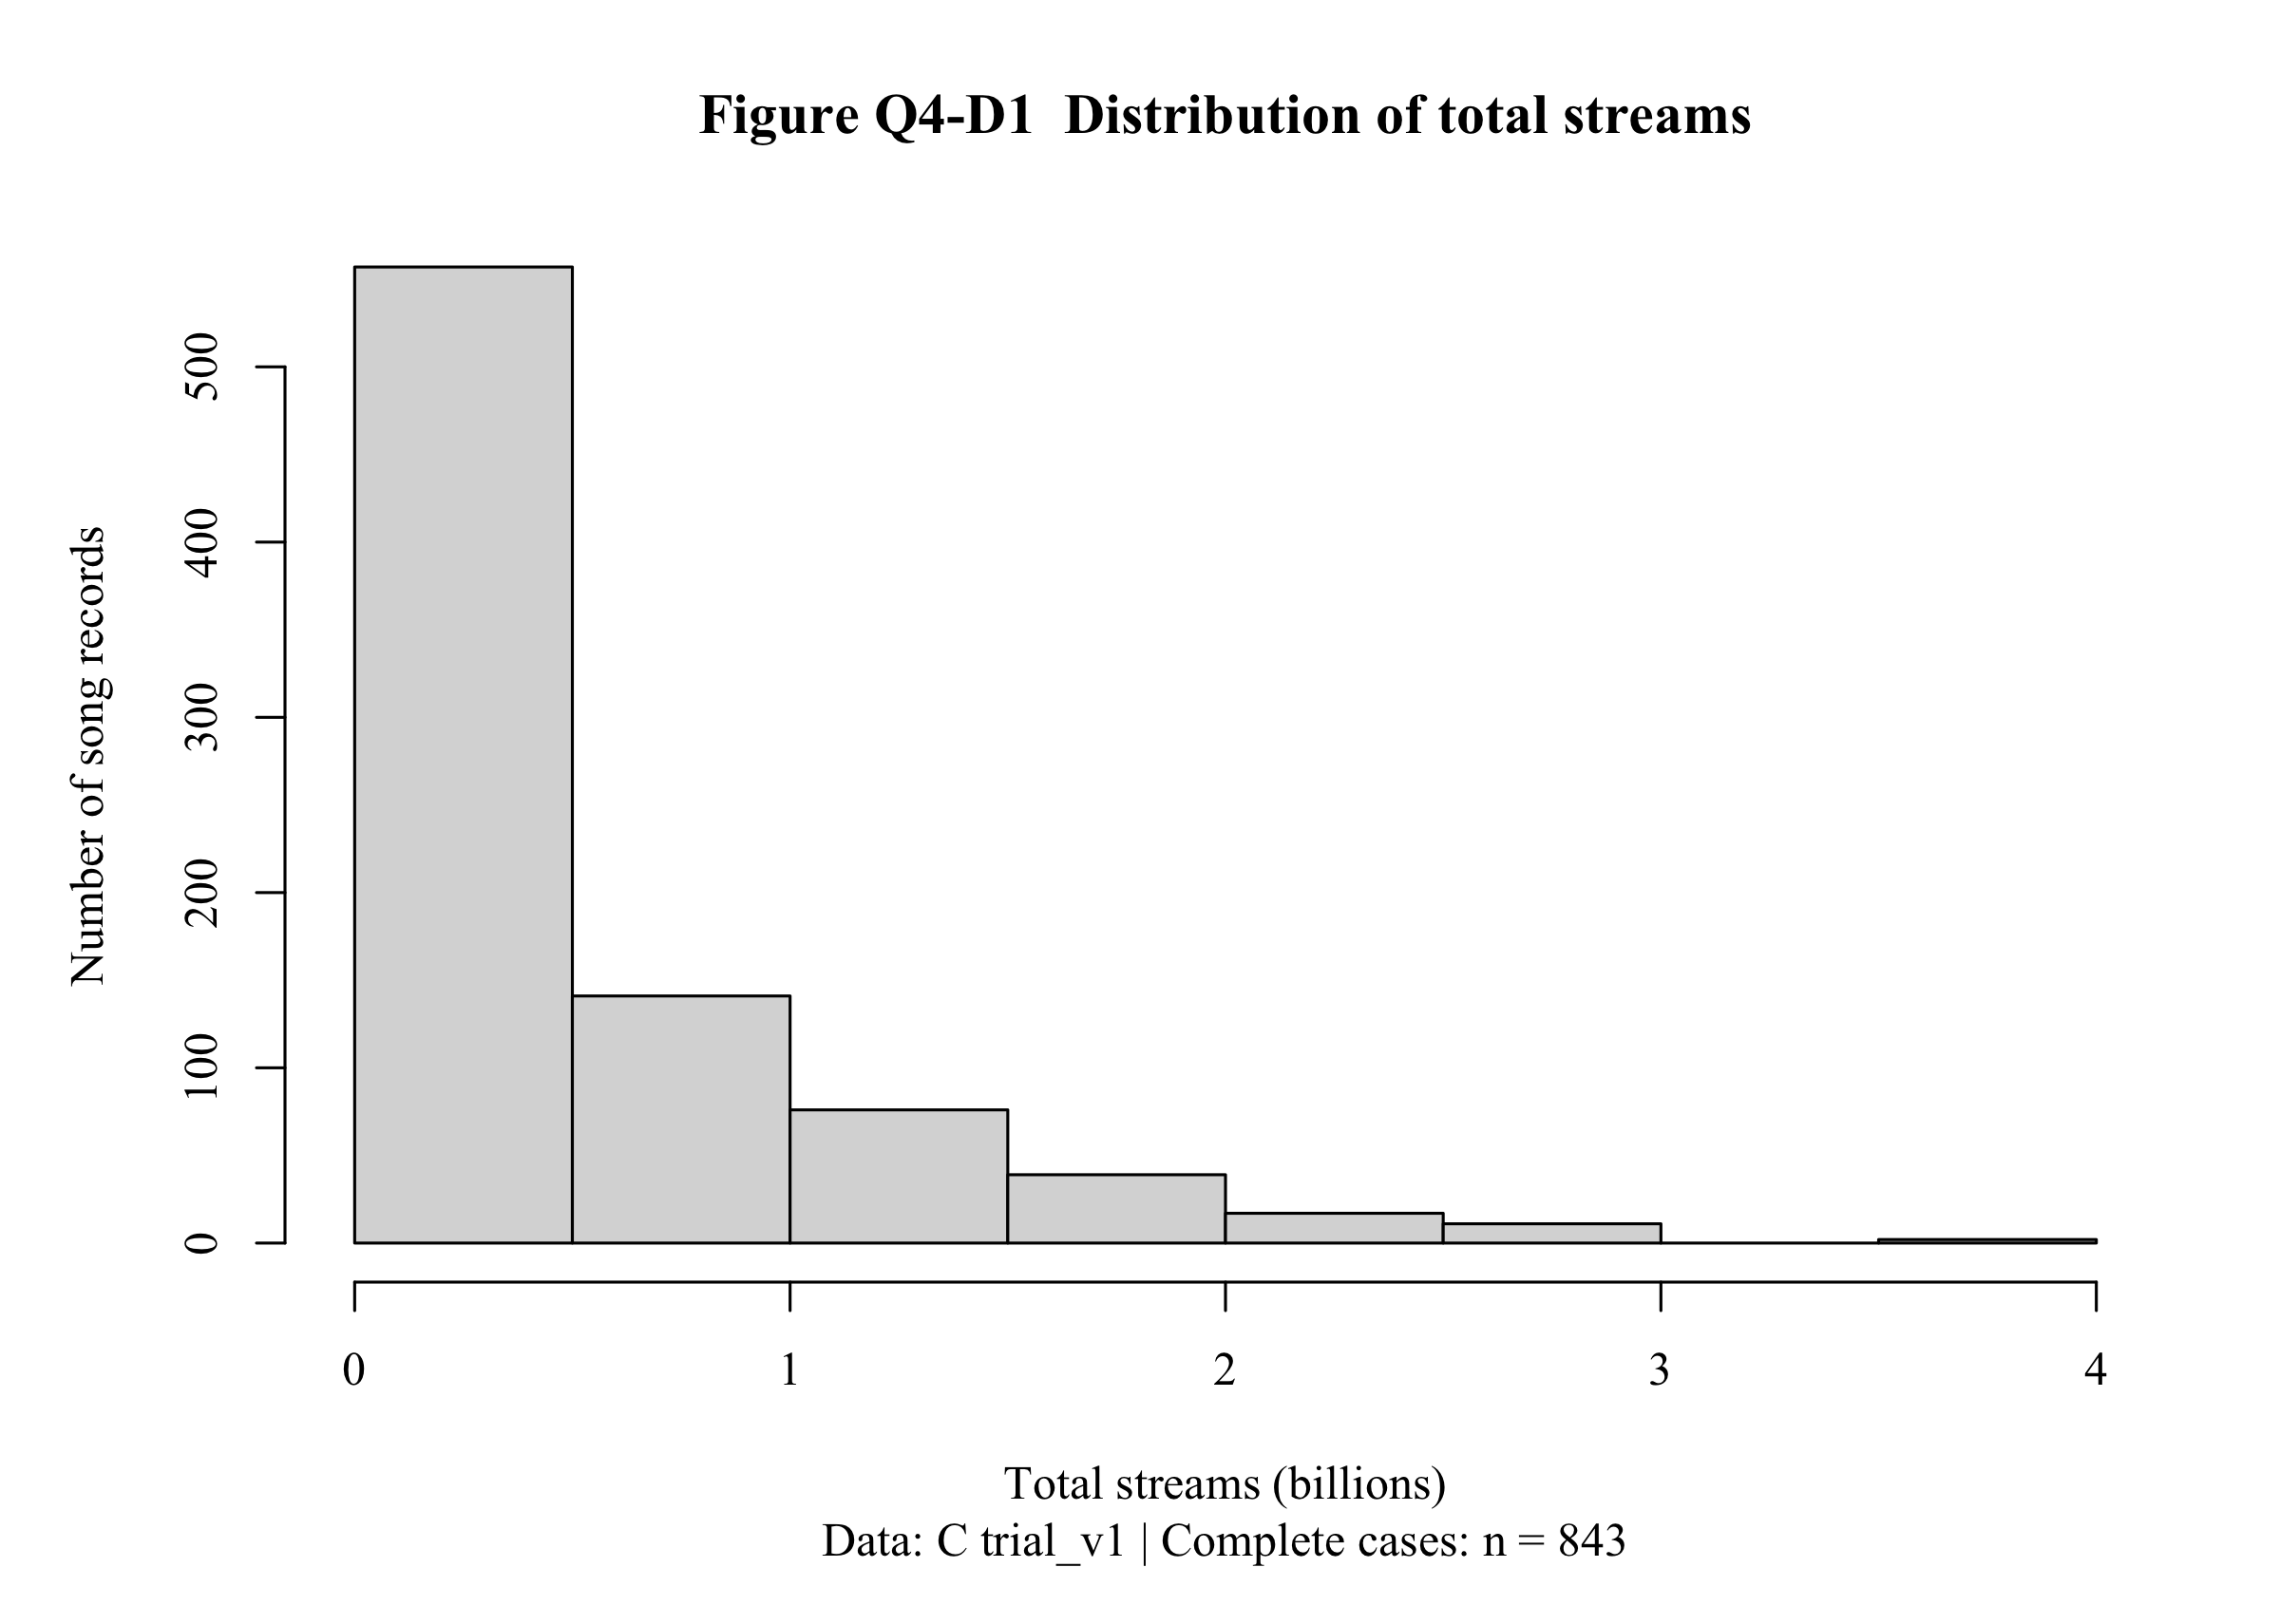
\includegraphics[width=0.8\textwidth]{Q4_D_Figure_01.png}
  \caption*{Figure Q4-D1: Distribution of total streams.}
\end{figure}

\begin{figure}[htbp]
  \centering
  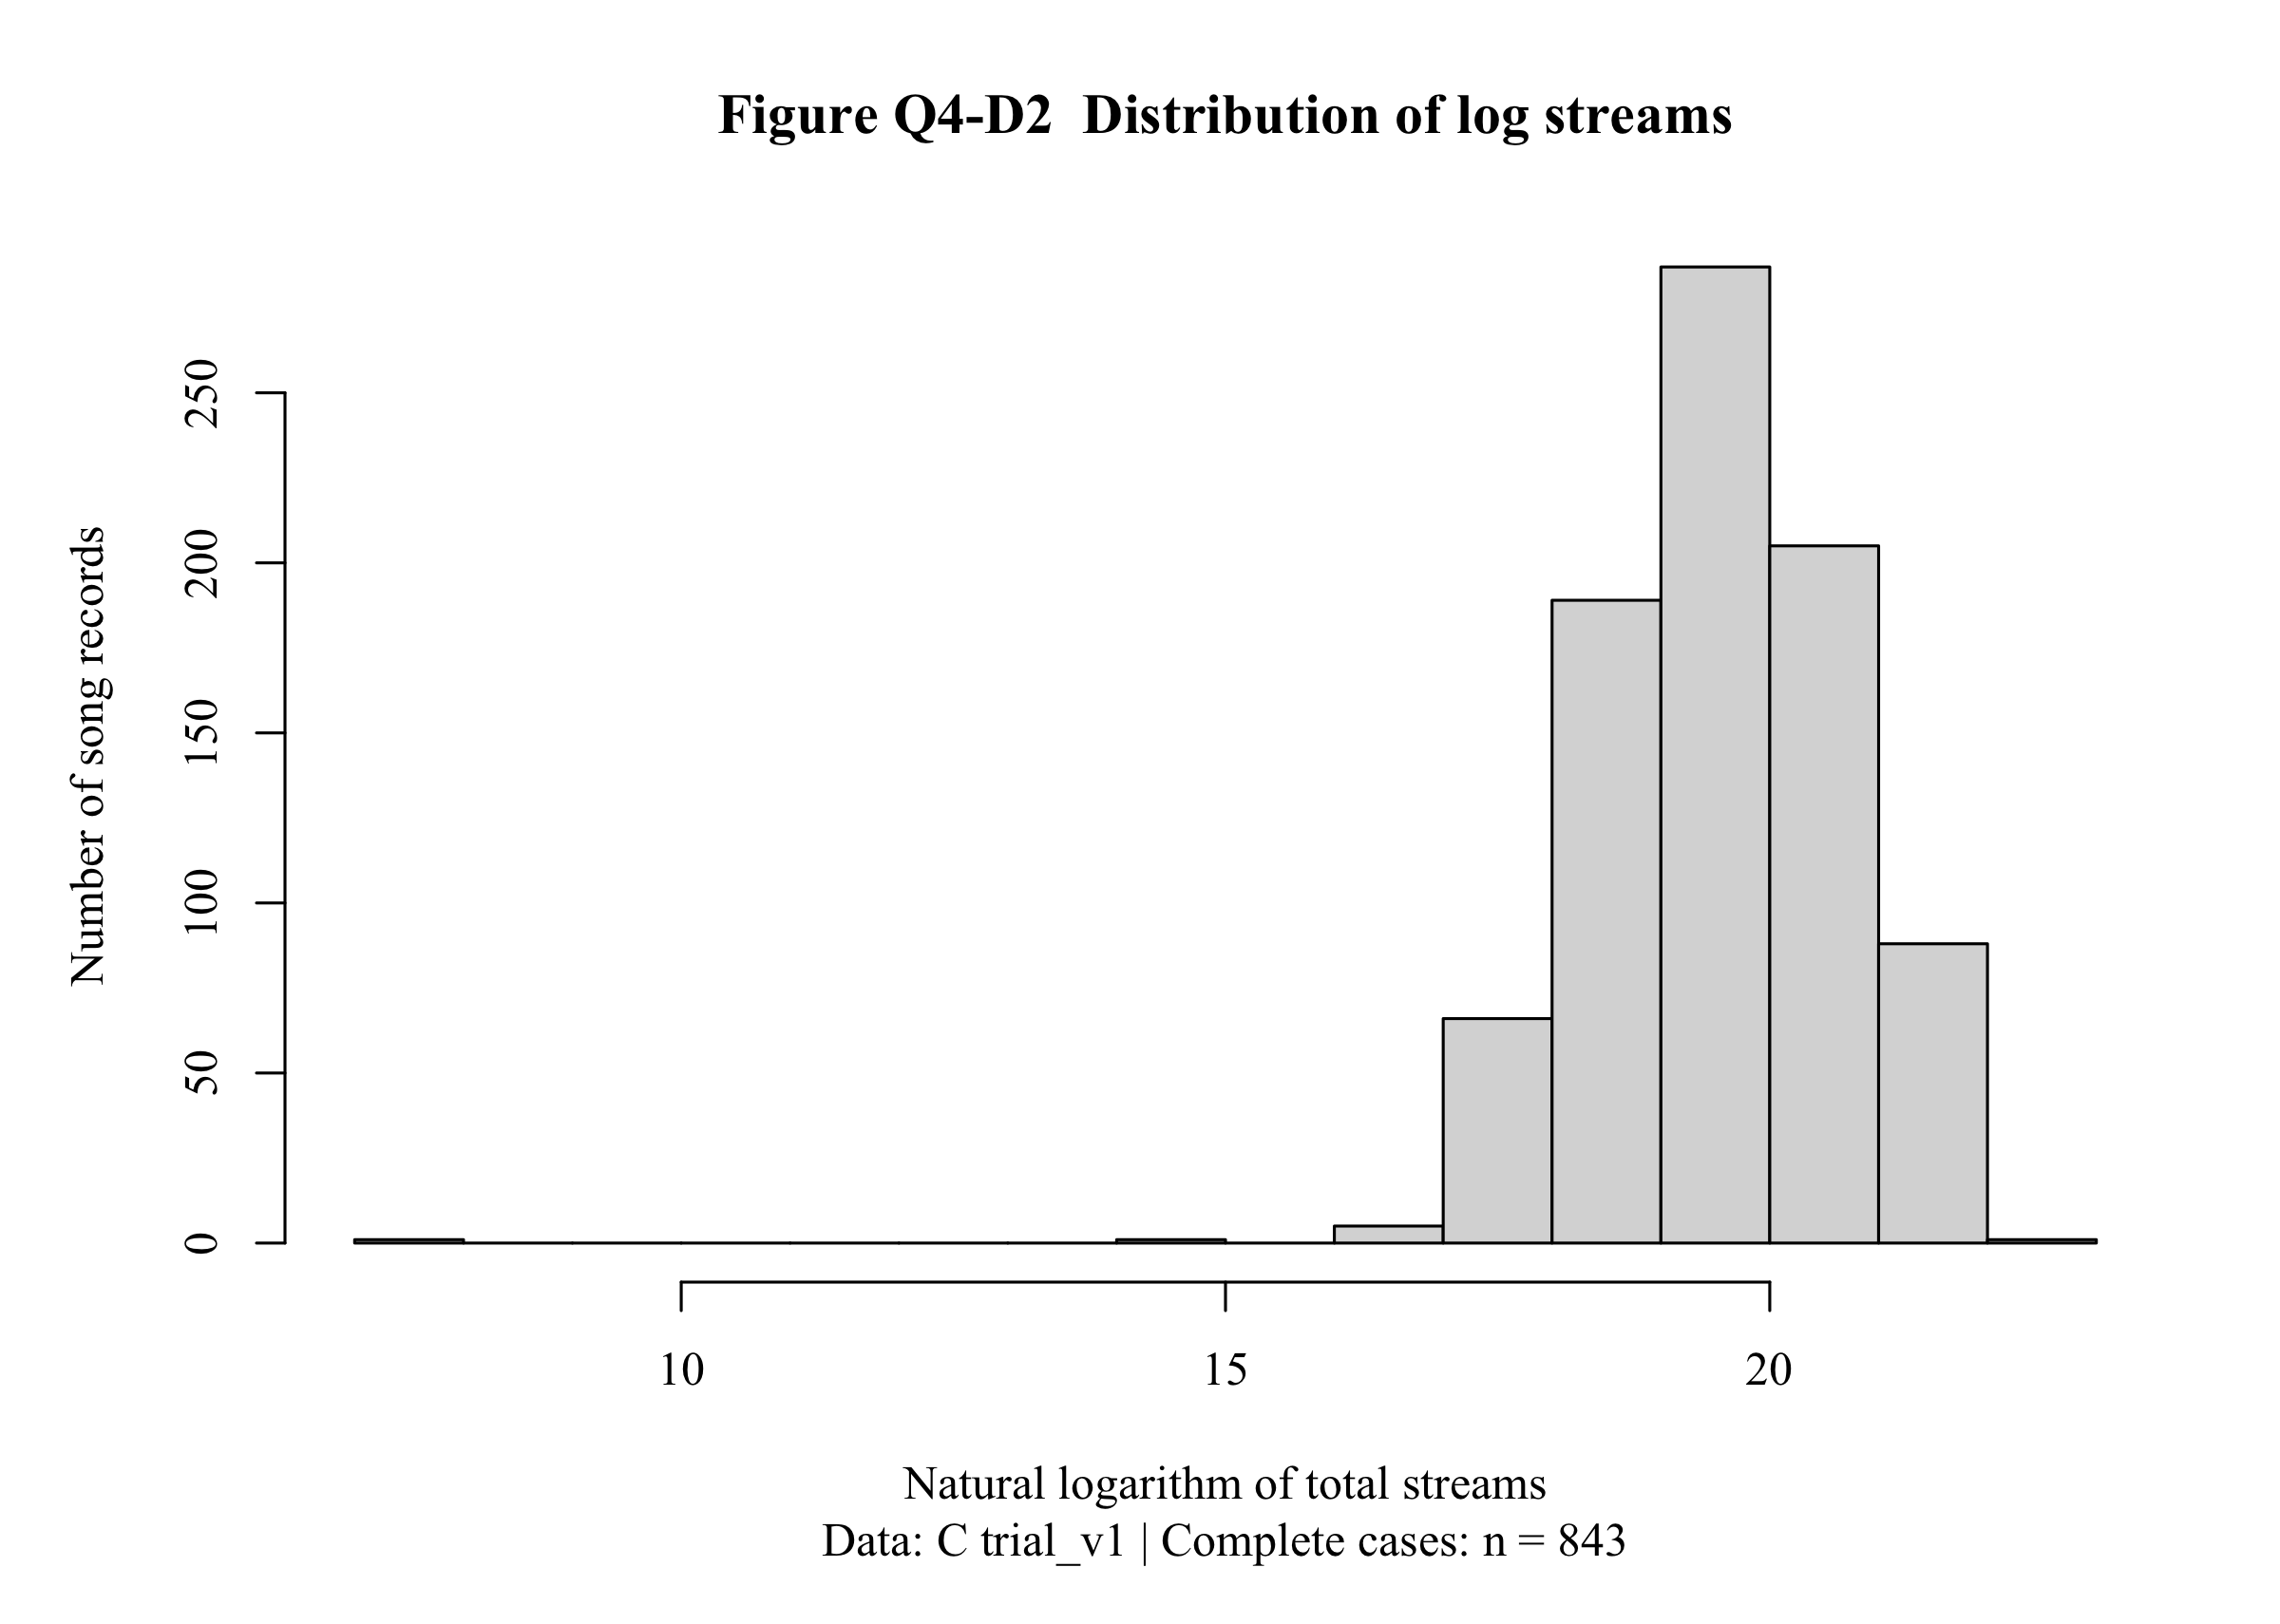
\includegraphics[width=0.8\textwidth]{Q4_D_Figure_02.png}
  \caption*{Figure Q4-D2: Distribution of log streams.}
\end{figure}

Figure Q4-D3 shows a positive but curved association between QQ playlist inclusions and log streams. The pattern is steeper at lower playlist counts and flatter at higher ones. When playlist inclusions are also transformed using the natural logarithm, the main pattern resembles a positive straight line more closely (see Figure Q4-D4). This suggests that log playlist inclusions should be considered in the candidate model. However, it does not establish the adjusted association, so model comparison and residual diagnostics are still needed.

\begin{figure}[htbp]
  \centering
  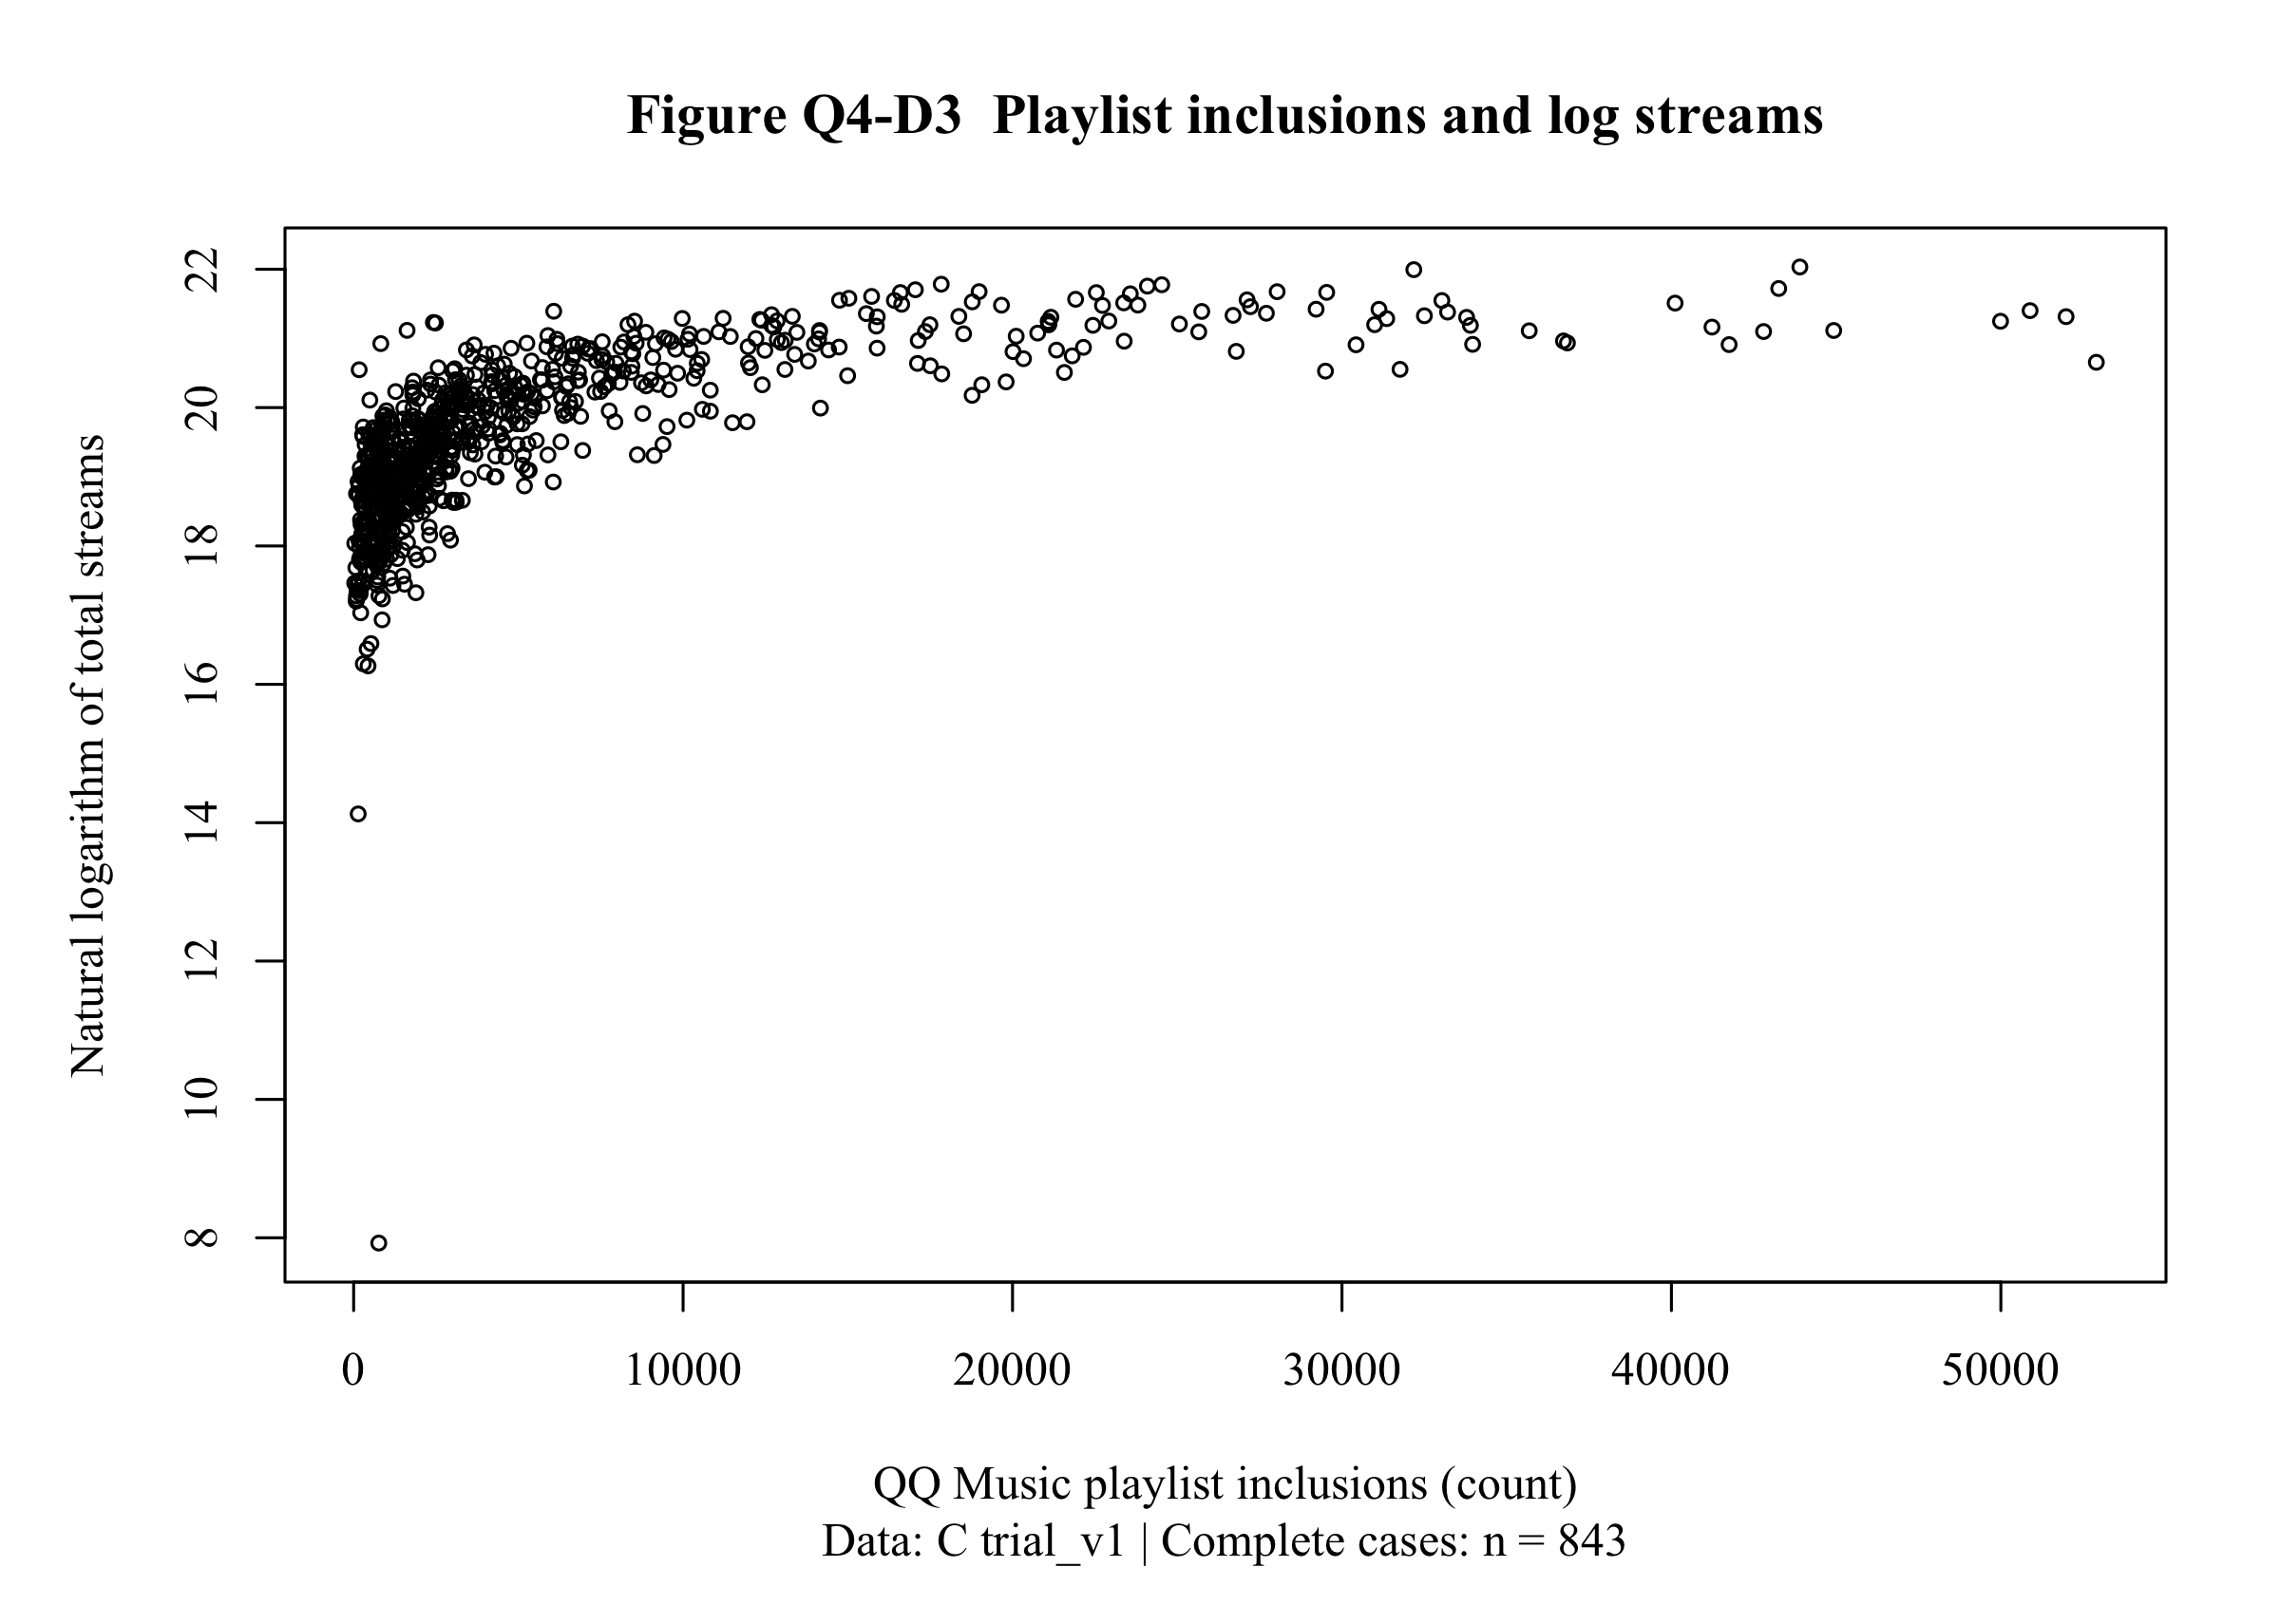
\includegraphics[width=0.8\textwidth]{Q4_D_Figure_03.png}
  \caption*{Figure Q4-D3: QQ playlist inclusions and log streams.}
\end{figure}

\begin{figure}[htbp]
  \centering
  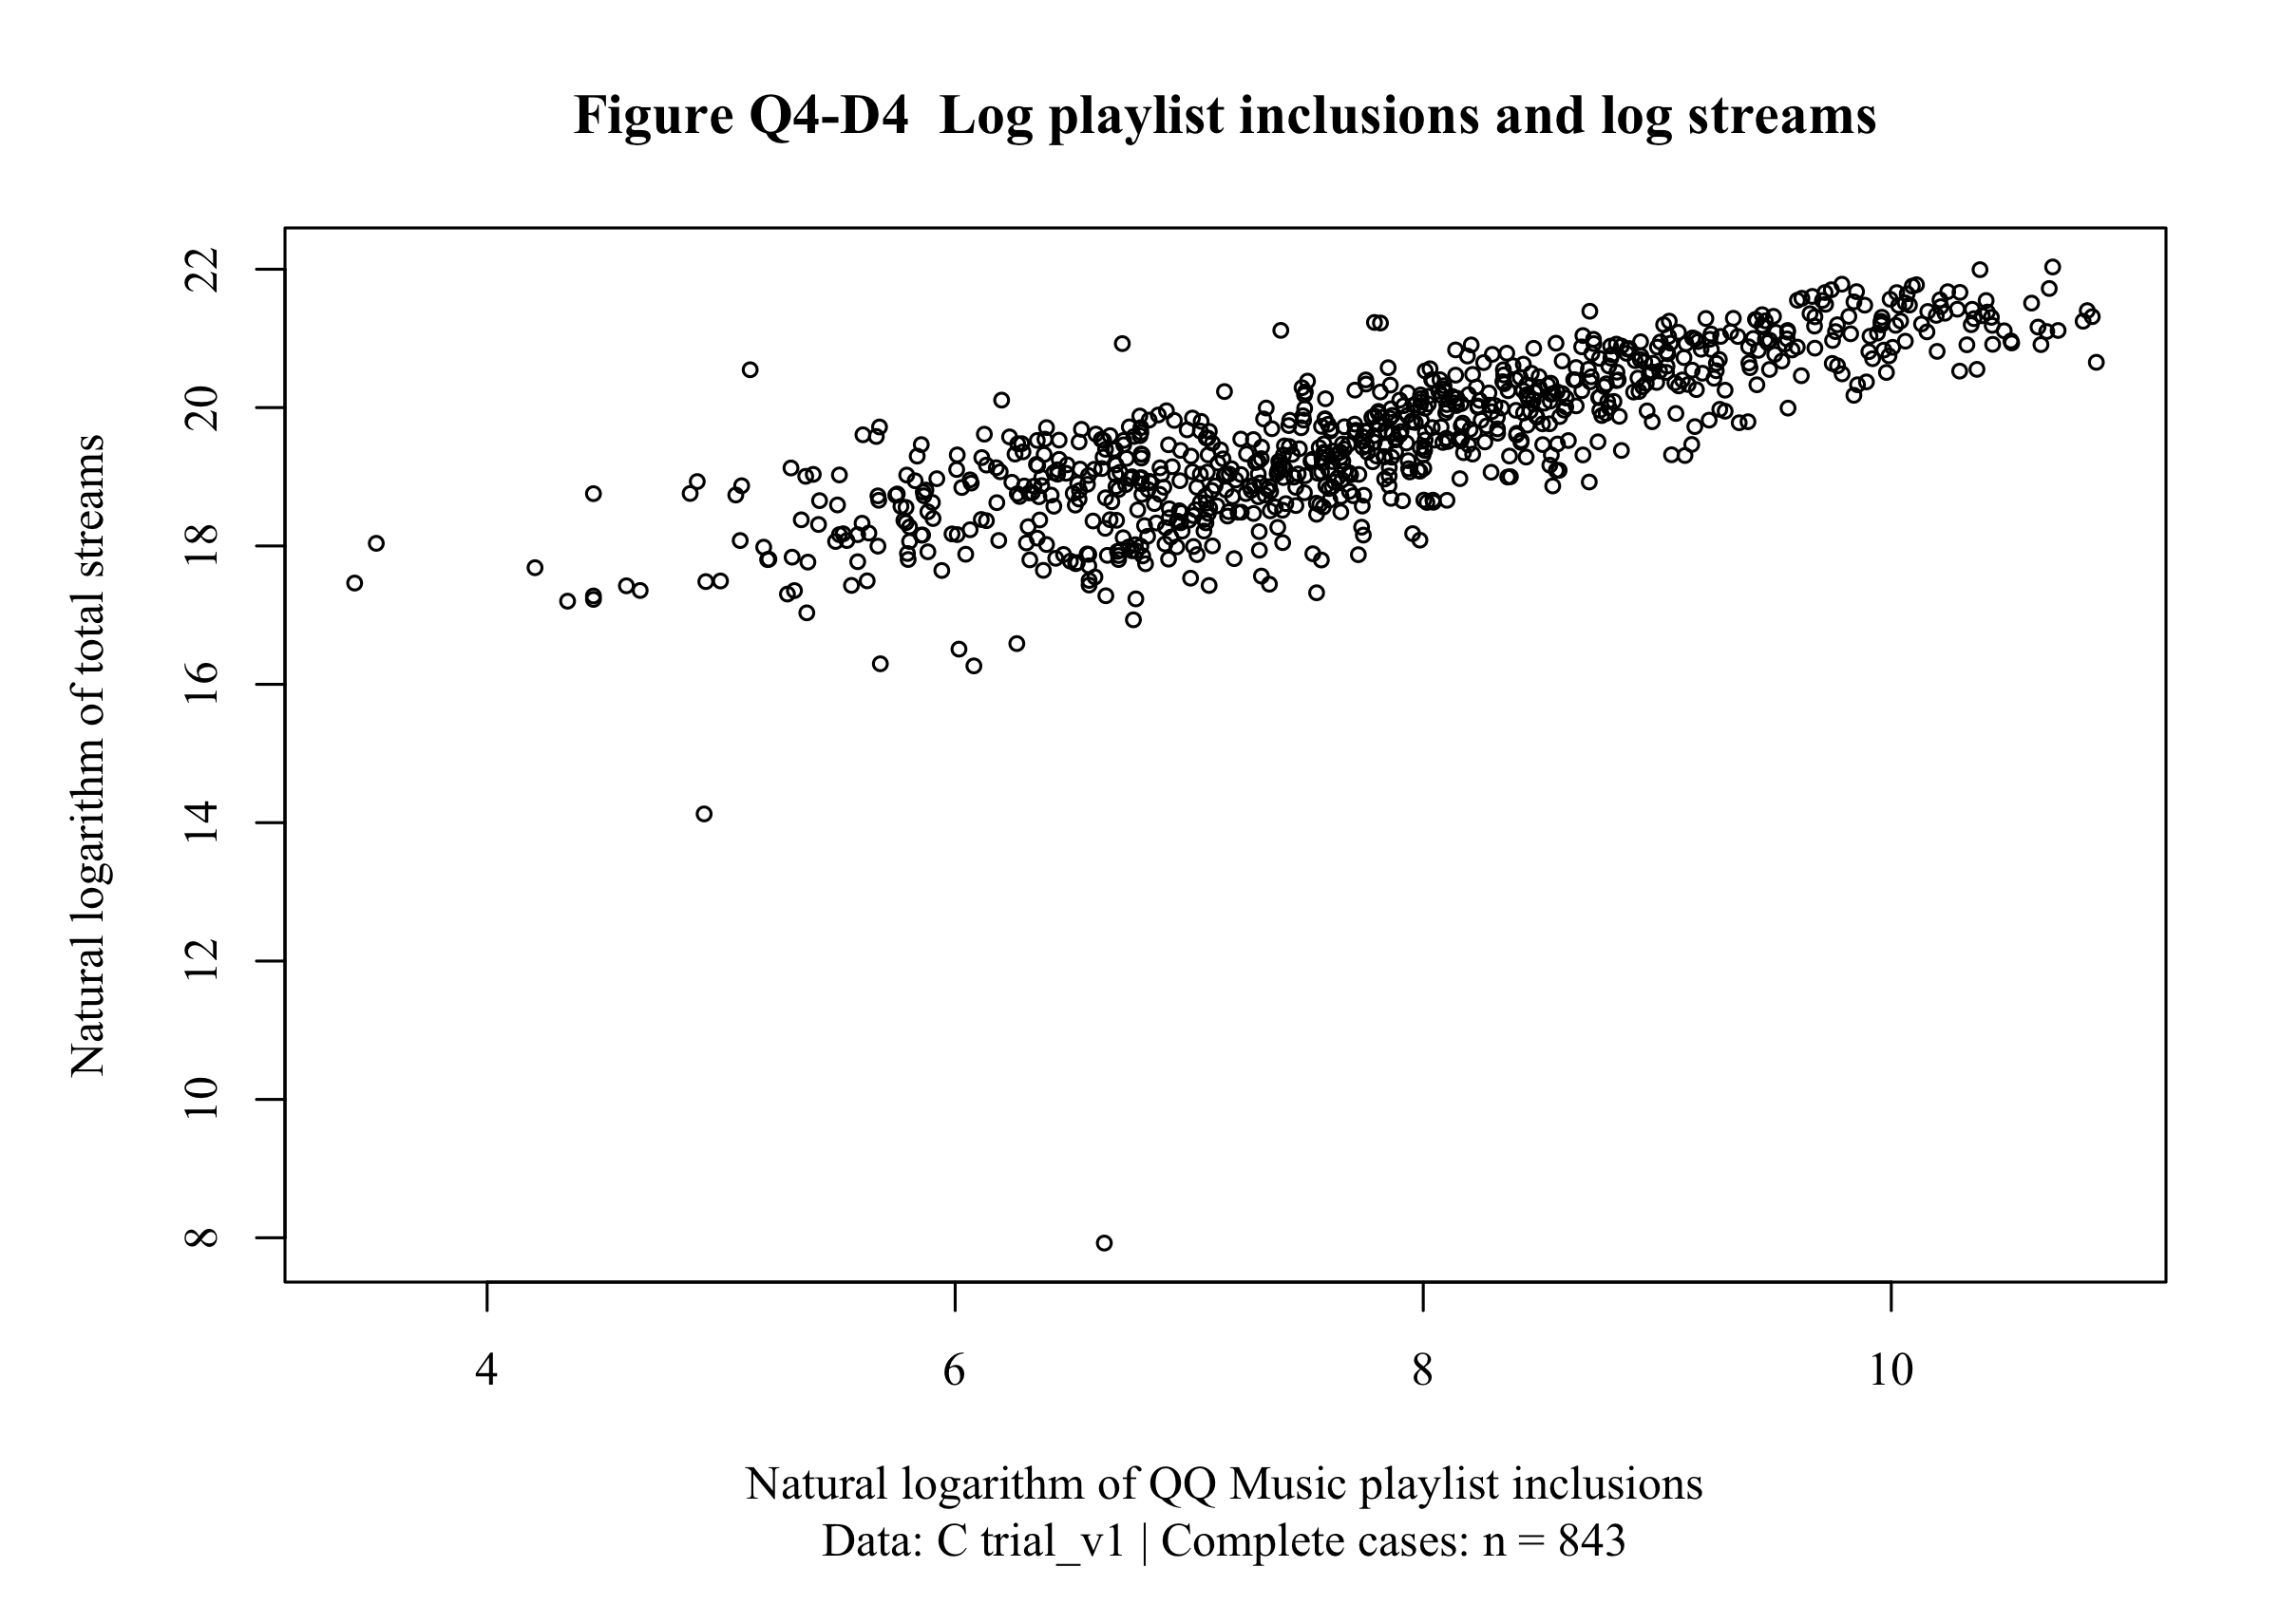
\includegraphics[width=0.8\textwidth]{Q4_D_Figure_04.png}
  \caption*{Figure Q4-D4: Log playlist inclusions and log streams.}
\end{figure}

Figure Q4-D5 shows a negative association between energy and acousticness. Their Pearson correlation is $-0.595$. Table Q4-D1 shows that the median values are 68.000 for danceability, 65.000 for energy and 17.000 for acousticness. These features are recorded on 0--100 scales. While these results describe the sample, they do not demonstrate that any feature causes higher streams.

\begin{figure}[htbp]
  \centering
  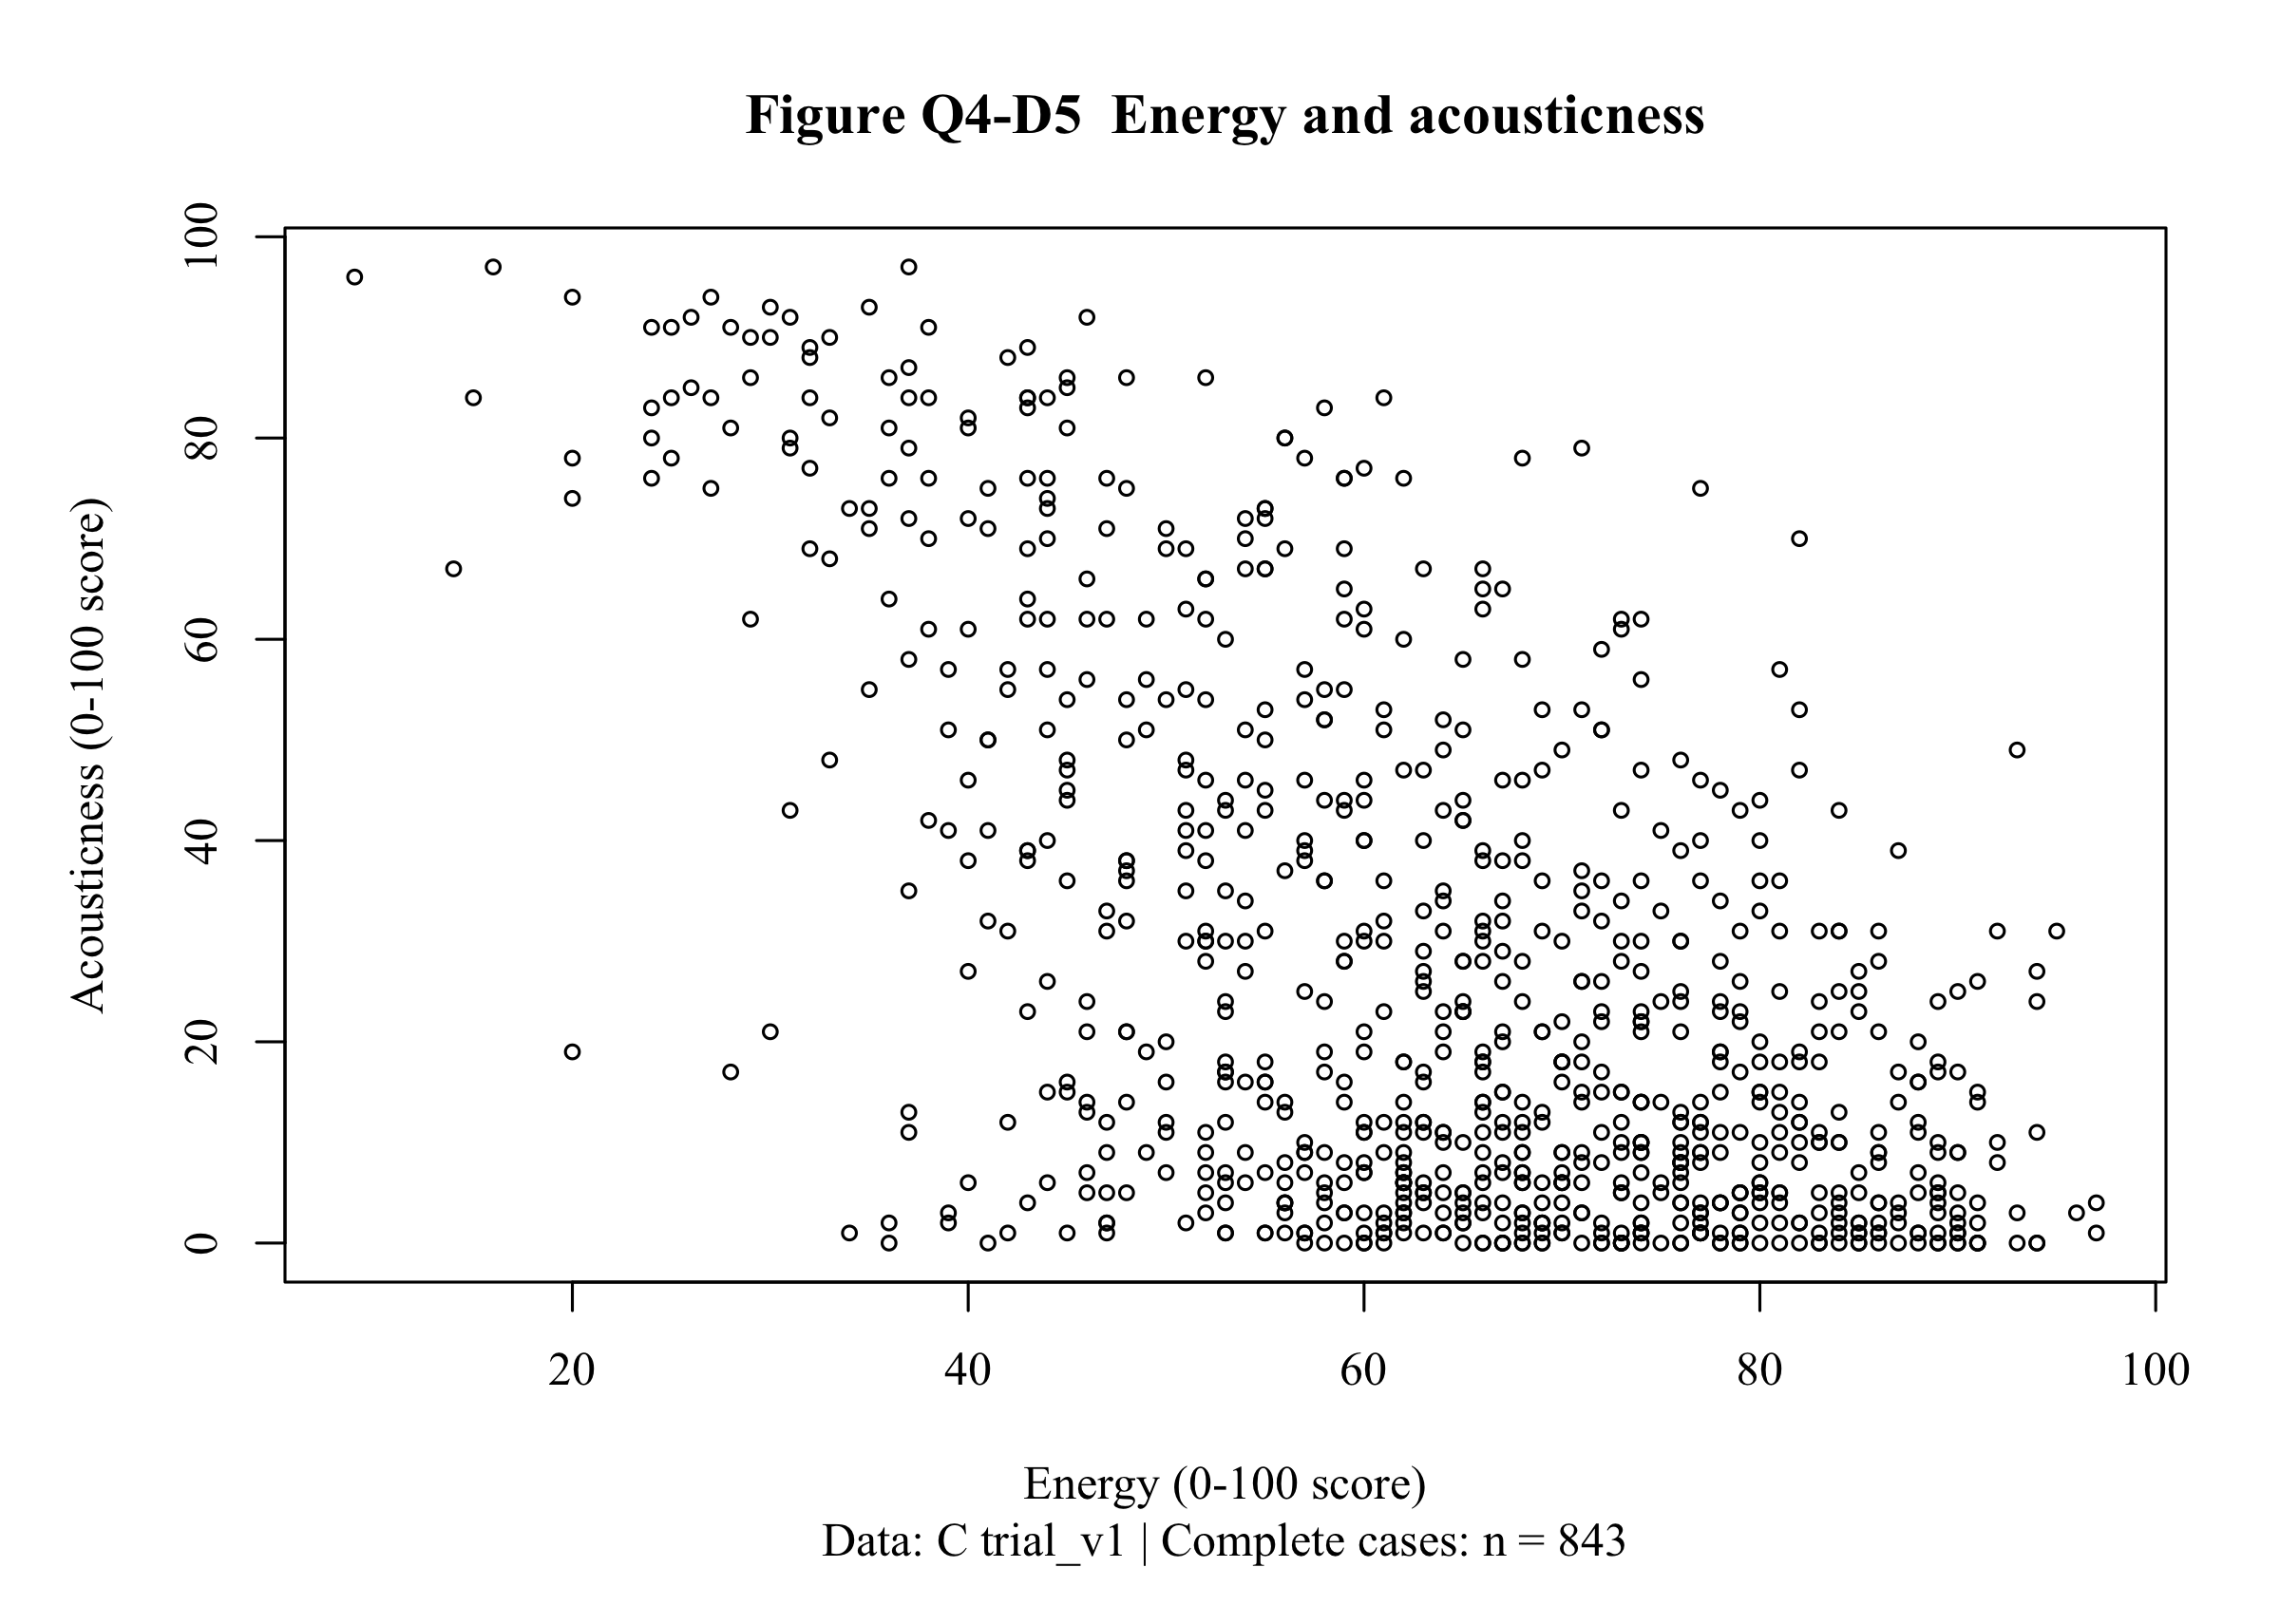
\includegraphics[width=0.8\textwidth]{Q4_D_Figure_05.png}
  \caption*{Figure Q4-D5: Energy and acousticness.}
\end{figure}

\subsection*{4.1(b) Research question and relevance}

Our research question is: How is QQ Music playlist inclusion associated with the natural logarithm of cumulative song streams, after accounting for artist count, release year, danceability, energy and acousticness?

The response variable is log(streams). QQ playlist inclusion is the main predictor, with its log transformation supported by the exploratory plots. The other candidate predictors are artist count, release year, danceability, energy, and acousticness. Playlist inclusion is important to the QQ Music team as a source of exposure. Studying its association with streams while accounting for selected song characteristics can inform the evaluation of playlist promotion. However, popular songs may also be more likely to be included in playlists. Therefore, the observed association cannot be interpreted as the effect of adding a song to a playlist.

% q4_variables.tex - Question 4 part 2 (OWNER: C) - prose integrated verbatim from docs/C_Q4_variable_roles.md
\subsection*{4.2 Variable Types and Analytical Roles}

Our research question is whether QQ Music playlist inclusion is associated with song streams after accounting for artist count, release year, danceability, energy and acousticness. Each observation is one song record. We use \texttt{log(streams)} as the response and \texttt{log(in\_QQ\_playlists)} as the main predictor. In R, \texttt{log()} denotes the natural logarithm.

\begin{table}[htbp]
  \centering
  \small
  \caption*{Table Q4-C1: Variable types and analytical roles.}
  \setlength{\tabcolsep}{3.5pt}
  \begin{tabular}{p{2.9cm}p{5.4cm}p{2.1cm}p{4.3cm}}
    \toprule
    Variable & Data type and measurement scale & Independent / dependent & Predictor / response \\
    \midrule
    \texttt{streams} & Quantitative, discrete count; ratio scale & Dependent & Response, entered as \texttt{log(streams)} \\
    \texttt{in\_QQ\_playlists} & Quantitative, discrete count; ratio scale & Independent & Main predictor, entered as \texttt{log(in\_QQ\_playlists)} \\
    \texttt{artist\_count} & Quantitative, discrete count; ratio scale & Independent & Candidate predictor \\
    \texttt{released\_year} & Quantitative; interval scale & Independent & Candidate predictor \\
    \texttt{danceability\_\%} & Quantitative score from 0 to 100; approximately interval & Independent & Candidate predictor \\
    \texttt{energy\_\%} & Quantitative score from 0 to 100; approximately interval & Independent & Candidate predictor \\
    \texttt{acousticness\_\%} & Quantitative score from 0 to 100; approximately interval & Independent & Candidate predictor \\
    \bottomrule
  \end{tabular}
\end{table}

The original stream and playlist counts have meaningful zeros. Release year is interval-scaled because differences between years are meaningful, whereas ratios are not. The data dictionary defines the three audio features as scores, so we treat them as approximately interval rather than assuming that a score of 80 represents twice as much as 40. The log-transformed counts are analysed as continuous numerical variables; the table describes their original measurement scales.

Danceability, energy and acousticness were evaluated as candidate predictors in the full model. The selected model (m2) retained log playlist inclusions, artist count and release year. All candidate models used the same complete-case sample.

The current analysis uses 843 complete records from \texttt{QQ\_Music\_trial\_v1.csv}. The working dataset retains all 844 rows, with the invalid \texttt{streams} entry in source data row 509 recorded as \texttt{NA}. Records with blank \texttt{key} values are retained because \texttt{key} is not included. The four candidate duplicate pairs are also retained pending further review.

\texttt{track\_name} and \texttt{artist(s)\_name} are nominal labels used for checking record identity; neither is a predictor nor a response in this analysis. Independent and dependent refer to model roles and do not imply a causal relationship.

% q4_predictors.tex - Question 4 parts 3(a) 3(b) (OWNER: D) - prose integrated verbatim from report/Q4_D_report_final.md
\subsection*{4.3(a) Candidate predictor selection}

We included playlist inclusions as they are the main variable of interest. The log transformation reduces the curvature seen in Figure Q4-D3, making it a reasonable candidate for the model. As all observed playlist counts and non-missing stream counts are positive, no constant was added before taking logarithms.

We included artist count to account for differences between solo songs and collaborations. This variable ranges from 1 to 8, with a median of 1.000. Records involving many artists are sparse, so conclusions about these small groups require caution. The release year was included because earlier releases may have had more time to accumulate streams and playlist inclusions. Its median is 2022, with a range of 1942--2023. However, release year is not a direct measure of time spent on the platform.

Danceability describes suitability for dancing, energy describes perceived intensity, and acousticness describes acoustic character. Their observed ranges are 23--96, 9--97, and 0--97, respectively. We included these three features to account for selected differences in the songs themselves. The correlation and VIF checks do not indicate a need to remove them because of serious multicollinearity. Song and artist names are identifiers. We excluded key and other platform indicators to focus the analysis on the agreed question regarding QQ playlist inclusion. This is a scope decision and does not imply that those variables are unrelated to popularity.

\subsection*{4.3(b) Correlation and multicollinearity}

We calculated the Pearson correlations between the six numerical predictors, excluding the response variable (see Table Q4-D2). In this table, playlist inclusions are on the natural logarithm scale. The largest absolute pairwise correlation is between energy and acousticness, at $-0.595$. The correlation between log playlist inclusions and release year is $-0.397$. However, these results alone cannot rule out multicollinearity because a predictor can be related to several other predictors simultaneously.

\begin{table}[htbp]
  \centering
  \small
  \caption*{Table Q4-D2: Pearson correlations among the numerical predictors ($n = 843$).}
  \begin{tabular}{lrrrrrr}
    \toprule
     & \shortstack[l]{ln(QQ\\playlists)} & \shortstack[l]{Artist\\count} & \shortstack[l]{Release\\year} & Danceability & Energy & \shortstack[l]{Acoustic-\\ness} \\
    \midrule
    ln(QQ playlists)      & 1      & $-0.097$ & $-0.397$ & $-0.113$ & $-0.004$ & $-0.048$ \\
    Artist count          & $-0.097$ & 1      & 0.094    & 0.198    & 0.132    & $-0.120$ \\
    Release year          & $-0.397$ & 0.094 & 1        & 0.183    & 0.110    & $-0.137$ \\
    Danceability          & $-0.113$ & 0.198 & 0.183    & 1        & 0.200    & $-0.256$ \\
    Energy                & $-0.004$ & 0.132 & 0.110    & 0.200    & 1        & $-0.595$ \\
    Acousticness          & $-0.048$ & $-0.120$ & $-0.137$ & $-0.256$ & $-0.595$ & 1 \\
    \bottomrule
  \end{tabular}
\end{table}

We therefore calculated the variance inflation factors for the candidate linear model containing the six predictors (see Table Q4-D3). The VIFs range from 1.058 to 1.627. The regression lecture identifies values around or above 5 as indicating the need to examine collinearity. All of our values are below 2, so these diagnostics do not indicate serious multicollinearity in this candidate model. We will not remove any of the six predictors solely because of multicollinearity. This does not establish that the model is optimal or that its other assumptions are satisfied.

\begin{table}[htbp]
  \centering
  \caption*{Table Q4-D3: Variance inflation factors for the candidate model with six predictors.}
  \begin{tabular}{lr}
    \toprule
    Variable & VIF \\
    \midrule
    ln(QQ playlists) & 1.215 \\
    Artist count & 1.058 \\
    Release year & 1.239 \\
    Danceability & 1.133 \\
    Energy & 1.563 \\
    Acousticness & 1.627 \\
    \bottomrule
  \end{tabular}
\end{table}

% q4_models.tex - Question 4 parts 3(c) 3(d) 3(e) (OWNER: E) - prose integrated verbatim from report/Q4_E_report_final.md
\subsection*{4.3(c) Model specification and selection}

The response log(streams) is continuous and approximately symmetric after the log transformation shown in Figure Q4-D2, so we fitted generalized linear models with the Gaussian family and identity link using \texttt{glm()}; this is equivalent to ordinary linear regression on the log scale. Following the research question, we compared three nested candidate models:

\begin{itemize}
  \item m1: $\log(\text{streams}) \sim \log(\text{in\_QQ\_playlists})$
  \item m2: $\log(\text{streams}) \sim \log(\text{in\_QQ\_playlists}) + \text{artist\_count} + \text{released\_year}$
  \item m3: $\log(\text{streams}) \sim \log(\text{in\_QQ\_playlists}) + \text{artist\_count} + \text{released\_year} + \text{danceability\_\%} + \text{energy\_\%} + \text{acousticness\_\%}$
\end{itemize}

Adding artist count and release year improves fit significantly (nested F test: $F = 9.288$, $\pval < 0.001$), whereas adding the three audio features does not ($F = 0.842$, $\pval = 0.471$). The AIC agrees: 1876.172, 1861.700 and 1865.156 for m1, m2 and m3 respectively (Table Q4-E1), so m2 is preferred by both criteria. The final model is therefore

\[
\log(\text{streams}) = 3.157 + 0.689 \cdot \log(\text{in\_QQ\_playlists}) - 0.114 \cdot \text{artist\_count} + 0.006 \cdot \text{released\_year},
\]

fitted on $n = 843$ songs with residual deviance 443.92 on 839 degrees of freedom ($R^2 = 0.614$). Variance inflation factors for the final model are at most 1.192 (Table Q4-E4), consistent with D's candidate-set check of 1.058 to 1.627, so multicollinearity is not a concern.

\begin{table}[htbp]
  \centering
  \caption*{Table Q4-E1: Model comparison by AIC.}
  \begin{tabular}{llr}
    \toprule
    Model & Specification & AIC \\
    \midrule
    m1 & log\_playlists & 1876.172 \\
    m2 & + artist\_count + released\_year & 1861.700 \\
    m3 & + danceability + energy + acousticness & 1865.156 \\
    \bottomrule
  \end{tabular}
\end{table}

Two coefficients in context. First, the elasticity of playlist inclusion is 0.689 (95\% CI $[0.649,\ 0.729]$, $t = 33.790$, $\pval < 0.001$): each 1\% increase in the number of QQ Music playlists including a song is associated with an approximately 0.689\% higher geometric-mean stream count, holding artist count and release year fixed; doubling playlist inclusions corresponds to a multiplicative factor of $2^{0.689} \approx 1.616$, i.e.\ about 61.6\% higher streams. Second, each additional contributing artist is associated with a multiplicative factor of $e^{-0.114} \approx 0.892$ (95\% CI for the coefficient $[-0.173,\ -0.055]$, $\pval < 0.001$), that is, about 10.8\% lower streams for collaborations of a given playlist exposure and release year. The release-year coefficient is small and positive (0.006, 95\% CI $[0.001,\ 0.010]$, $\pval = 0.025$); we interpret it cautiously because release year is an imperfect proxy for time available to accumulate streams. The elasticity estimate is essentially unchanged across m1, m2 and m3 (0.678, 0.689 and 0.692; Table Q4-E2), so the adjusted association between playlist inclusion and streams is robust to which controls enter the model.

\begin{table}[htbp]
  \centering
  \caption*{Table Q4-E2: Elasticity of log playlist inclusions across candidate models.}
  \begin{tabular}{lrr}
    \toprule
    Model & log\_playlists coefficient & $R^2$ \\
    \midrule
    m1 & 0.678 & 0.606 \\
    m2 & 0.689 & 0.614 \\
    m3 & 0.692 & 0.615 \\
    \bottomrule
  \end{tabular}
\end{table}

\begin{table}[htbp]
  \centering
  \small
  \caption*{Table Q4-E3: Final model (m2) coefficients with 95\% confidence intervals.}
  \begin{tabular}{lrrrrrr}
    \toprule
    Term & Estimate & SE & $t$ & $\pval$ & 2.5\% & 97.5\% \\
    \midrule
    (Intercept) & 3.157 & 5.051 & 0.625 & 0.532 & $-6.744$ & 13.057 \\
    log\_playlists & 0.689 & 0.020 & 33.790 & $< 0.001$ & 0.649 & 0.729 \\
    artist\_count & $-0.114$ & 0.030 & $-3.811$ & $< 0.001$ & $-0.173$ & $-0.055$ \\
    released\_year & 0.006 & 0.002 & 2.245 & 0.025 & 0.001 & 0.010 \\
    \bottomrule
  \end{tabular}
\end{table}

\begin{table}[htbp]
  \centering
  \caption*{Table Q4-E4: Variance inflation factors for the final model (m2).}
  \begin{tabular}{lr}
    \toprule
    Term & VIF \\
    \midrule
    log\_playlists & 1.192 \\
    artist\_count & 1.013 \\
    released\_year & 1.192 \\
    \bottomrule
  \end{tabular}
\end{table}

\subsection*{4.3(d) Diagnostics and prediction}

Figure Q4-E1 shows the four standard residual plots for the final model. Residuals against fitted values show no remaining systematic curvature, supporting the linearity of the log-log specification. The normal Q-Q plot is close to linear in the centre with somewhat heavier tails, which is common for large observational datasets; the residual-vs-log-playlists plot (Figure Q4-E2) shows no trend in location or spread across the observed range of playlist inclusions. The scale-location plot shows mildly increasing spread at high fitted values, indicating mild heteroscedasticity rather than a structural failure. The largest Cook's distance is 0.184 (``Dream On''), with all values far below levels that would indicate a single influential observation, so no records were removed.

\begin{figure}[htbp]
  \centering
  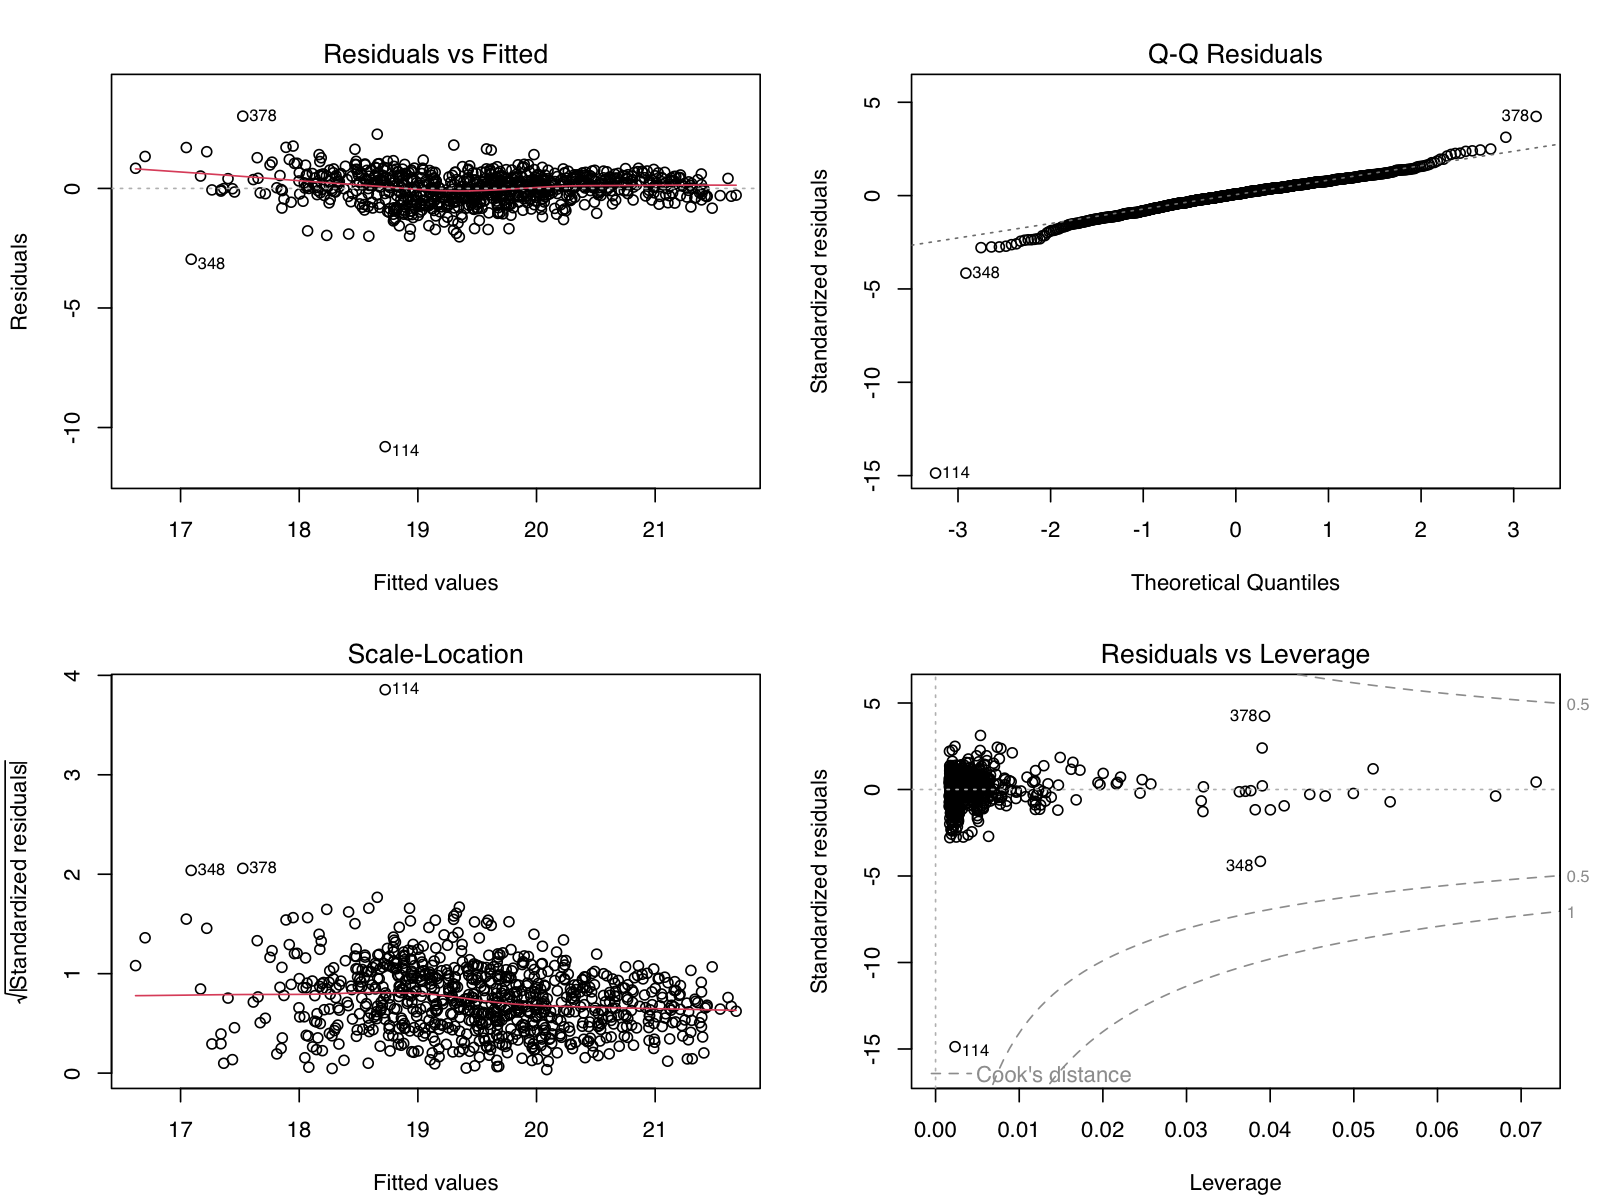
\includegraphics[width=0.9\textwidth]{Q4_E_Figure_01_diagnostics.png}
  \caption*{Figure Q4-E1: The four standard residual plots for the final model.}
\end{figure}

\begin{figure}[htbp]
  \centering
  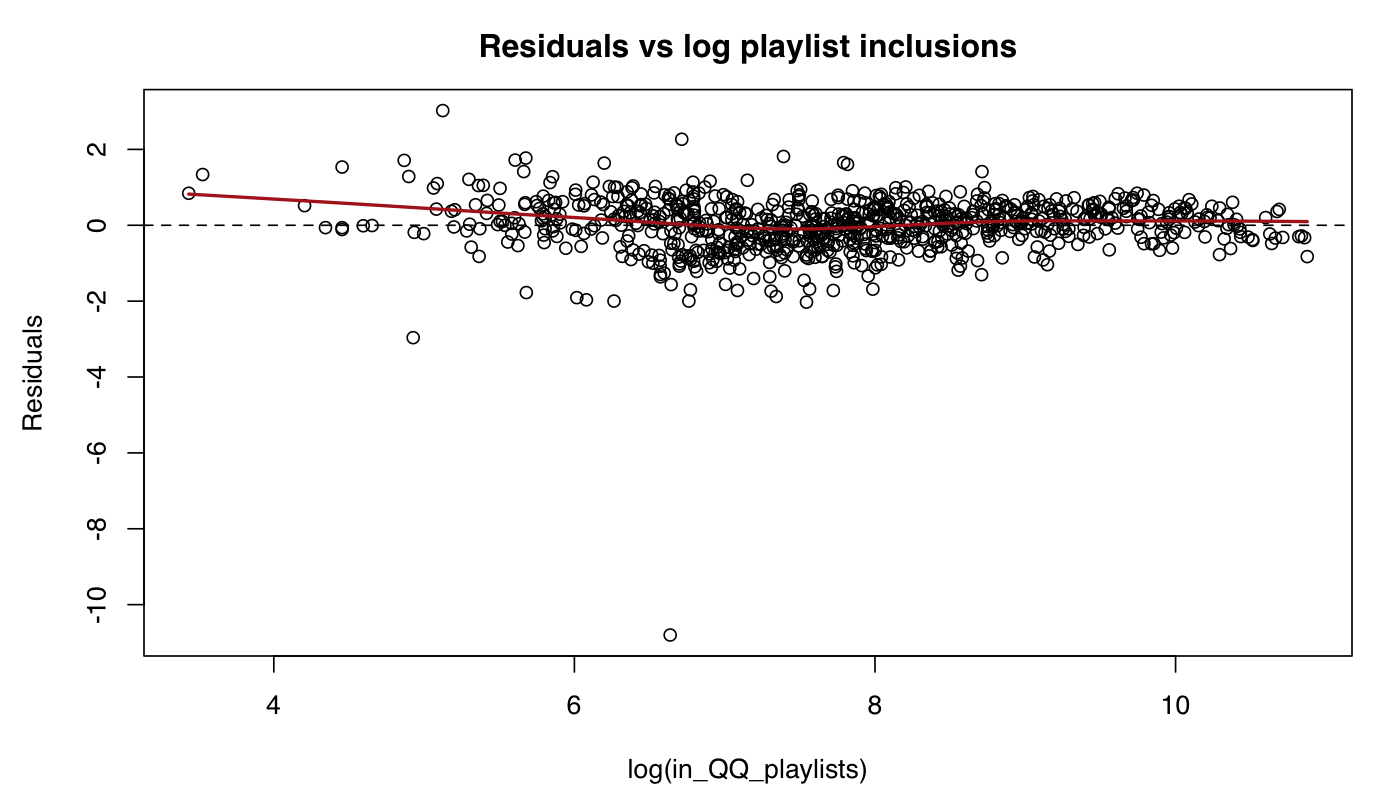
\includegraphics[width=0.85\textwidth]{Q4_E_Figure_02_residual_vs_log_playlists.png}
  \caption*{Figure Q4-E2: Residuals versus log playlist inclusions.}
\end{figure}

For prediction we defined a plausible scenario within the observed predictor ranges: a song included in the median number of playlists (2,313), with the median artist count (1) and median release year (2022). The predicted mean log streams is 19.606. The 95\% confidence interval for the mean response is $[306.753,\ 346.730]$ million streams: with 95\% confidence, the average log streams of songs with these characteristics lies in this range on the original scale. The 95\% prediction interval for a single new song with these characteristics is much wider, $[78.281,\ 1358.702]$ million streams, because it additionally accounts for song-to-song variability; the width of this interval reflects the large residual variation in individual streaming outcomes.

\begin{table}[htbp]
  \centering
  \small
  \caption*{Table Q4-E5: Prediction at the median scenario (playlists $= 2313$, artist count $= 1$, release year 2022).}
  \begin{tabular}{lll}
    \toprule
    Quantity & Interval, log scale & Interval, million streams \\
    \midrule
    Mean response CI & $[19.542,\ 19.664]$ & $[306.753,\ 346.730]$ \\
    New observation PI & $[18.176,\ 21.030]$ & $[78.281,\ 1358.702]$ \\
    \bottomrule
  \end{tabular}
\end{table}

\subsection*{4.3(e) Conclusion and model justification}

We answered the research question with a Gaussian GLM on log(streams), selecting the final model by nested F tests and AIC among three candidates that progressively added artist count and release year, then the three audio features. Both criteria preferred the model with playlist inclusion, artist count and release year (AIC $= 1861.700$); the audio features added no significant improvement ($\pval = 0.471$) and did not change the substantive conclusion.

The central finding is a strong, robust positive adjusted association between playlist inclusion and streams: the elasticity is 0.689 (95\% CI $[0.649,\ 0.729]$), stable at 0.678--0.692 across all candidate models, so songs included in more QQ Music playlists have substantially higher stream counts even after accounting for artist count, release year and audio characteristics. Collaborations are associated with about 10.8\% lower streams at equal playlist exposure. For the QQ Music team, this quantifies how strongly playlist reach tracks streaming performance and supports treating playlist placement as a key visibility lever, although reverse causality is plausible: popular songs are also more likely to be added to playlists.

Limitations: the data are observational, so coefficients describe associations rather than causal effects of playlist placement; unmeasured factors such as label promotion and artist fame may drive both inclusion and streams; release year imperfectly measures accumulation time; diagnostics indicate mildly heavy-tailed residuals and mild heteroscedasticity; and the wide prediction interval shows that individual song outcomes remain highly variable.

\section*{External Sources and AI-Assistance Disclosure}
\FloatBarrier
\subsection*{Data and software sources}
\begin{itemize}\setlength\itemsep{2pt}
\item \texttt{QQ\_Music.csv}: supplied with the assignment on the course Moodle page (Question 4).
\item \texttt{Hitters}, \texttt{College} and \texttt{Auto}: datasets in the \texttt{ISLR2} R package (Question 3); original descriptions are available through the package help pages.
\item \texttt{chickwts}: included in R's \texttt{datasets} package (Question 2).
\item R statistics and graphics, \texttt{ISLR2} and \texttt{car}; course materials on hypothesis testing, EDA and regression informed the analysis. Session information is retained with the analysis outputs.
\end{itemize}

For supplementary model selection and diagnostics, we consulted the R \texttt{stats} documentation for \texttt{AIC}, \texttt{anova.lm}, \texttt{lowess} and \texttt{influence.measures}, and the \texttt{car::vif} documentation. LOWESS is used only to display a descriptive residual trend. The Cook's-distance rule $4/n$ is an exploratory screening guideline, not a required course cutoff or an automatic deletion rule. These implementation details are not claimed to have appeared verbatim in the course slides.
\FloatBarrier
\subsection*{AI-assistance disclosure}
The following statements record the members' reported uses of assistance. Numerical analyses were generated in R and checked against the source data and outputs. These statements document usage; permission is governed by the course policy.
\begin{itemize}\setlength\itemsep{3pt}
\item \textbf{LING Tong:} AI assistance was used to help draft the report and explain errors in the R code.
\item \textbf{CHEN Yanwu:} AI assistance was used for code comments, report drafting, numerical checks, revisions and the Chinese reading translation. Analyses were checked by running R against the source datasets.
\item \textbf{CHEN Yinan:} AI assistance was used to help write and debug the R code and to draft and edit my sections of the report.
\item \textbf{ZHANG Yijie:} AI assistance was used to organise the analysis and draft explanations. DeepL Write was used for language revision. Numerical results were produced in R and independently checked.
\item \textbf{HU Zhongyuan:} AI assistance was used to help draft the report and explain errors in the R code.
\end{itemize}


\end{document}
